\chapter{Performance Assessment of Interface Components}
\label{ch:p1:performance}

\dictum[Tom Cargil]{%
    The first 90 percent of the code accounts for the first 90 percent of the development time. The remaining 10 percent of the code accounts for the other 90 percent of the development time. }%
\vskip 1em

\readit{2}

% \worktodo{
% this section need FULL refactoring!
% Performance assessment for (all without transfers)
% \begin{itemize}
%     \item[x] Quda dop, cstar and periodic on synthetic data on daint strong.
%     \item[x] Quda dop, cstar and periodic on synthetic data on daint weak.
%     \item openqxd Dirac operator cstar and periodic on synthetic data on daint strong.
%     \item[1/2] openqxd Dirac operator cstar and periodic on synthetic data on daint weak.
%     \item[1/2] openqxd deflated solver vs quda mg simple solver, strong and weak scaling with G8 (periodic) and D300 (cstar, qcd-only) and evtl. C380 (cstar and qcd-qed) on daint.
%     \item[x] quda simple solver vs. quda mrhs solver. Done: D300 and A400 speedup vs. nrhs (16 and 32)
%     \item[x] quda simple solver vs. quda async solver overlapping something (not yet sure what to overlap). Done: A360 at geno 1 node: good, A400 at daint 2 nodes: VERY bad, F7 at daint 1 node: BAD
%     \item[x] performance degradation of \code{MPI\_THREAD\_MULTIPLE}. Done: in previous plots.
%     \item[x] performance degradation of dual lattice (or contribution of inter-grid data movement to total). Dual lattice is very inefficient on daint-alps! Maybe rewrite such that only one MPIsend/recv per non-quda rank? Else it is infeasible I think
%     \item strong scaling inverter plot with: sync vs. async vs. dual on G8/D300/C380
%     \item[x] ideally activate GDR ...
%     \item ideally activate nvshmem ...
% \end{itemize}
% }

\tldr{intro}
This chapter will present performance assessments of the various implementations discussed in \cref{ch:p1:interface}.
The goal is to determine production readiness of the code to run on current accelerator-based super-computing centers, focusing on good performance on the very recent GH200 (Grace-Hopper) node at CSCS~\cite{fusco2024}.
All machines involved in data taking are specified in \cref{sec:perf:hardware}.
The physics program of the \RCstar collaboration is centered around lattices with \Cstar boundary conditions and occasionally periodic ones.
Thus, we ran performance tests on lattices specified in \cref{sec:perf:ensembles}, whereas the methodology of measurements is discussed in \cref{sec:perf:methodology}.
Among the investigated features were runtime contributions of the dual process grid (\cref{sec:perf:dual}), the efficiency of  heterogeneous workloads using the asynchronous solver with concurrent workload on the CPU (\cref{sec:perf:solver:async}), the blocked solver acting on multiple RHS at the same time (\cref{sec:perf:solver:mrhs}), asymptotic strong and weak scaling behavior of the Dirac operator (\cref{sec:perf:dop}) and finally scaling of multigrid solver as used in production (\cref{sec:perf:solver}).
The chapter ends with concluding remarks and limitations (\cref{sec:perf:summary}).

\section{Hardware specifications}
\label{sec:perf:hardware}

\newcommand{\datataking}[1]{The data was taken on \emph{#1}, see \cref{sec:perf:hardware}.}

\tldr{machine we ran on}
The performance measures that follow were obtained on the machines
\begin{itemize}
    \item \emph{Daint-Alps} at CSCS, Switzerland, 4\x NVIDIA\textsuperscript{\textregistered} Grace @ 3GHz (72 Arm Neoverse V2 cores), 4\x 128GB LPDDR memory, 4\x NVIDIA\textsuperscript{\textregistered} Tesla\textsuperscript{\textregistered} H100 (96GB HBM2 memory)
    \item \emph{Leonardo Booster} at CINECA, Italy, 1\x Intel\textsuperscript{\textregistered} Xeon\textsuperscript{\textregistered} Platinum 8358 @ 2.6 GHz (32 cores, Icelake), 8\x 64 GB DDR4-3200 memory, 4\x NVIDIA\textsuperscript{\textregistered} Ampere A100 (64GB HBM2 memory)~\cite{leonardo:booster}
    %\item \emph{Geno} at ETHZ, Switzerland, 2\x AMD EPYC\textsuperscript{\texttrademark} 9124 @ 3GHz (16 cores, Zen 4), 1.5 TB memory, 8\x NVIDIA\textsuperscript{\textregistered} RTX A2000 (12 GB GDDR6 memory)
\end{itemize}

The Quad GH200 node is an interesting machine, since it comes with many new concepts and a sophisticated memory hierarchy~\cite{fusco2024}.
All compute units (CPUs and GPUs) within the node are able to access each others memory directly, enabling zero-copy access.
This hierarchy of the unified address space is fully coherent and is abstracted with the help of individual NUMA domains.
The chips themselves are connected via NVLink-C2C, a high bandwidth low latency chip-to-chip interconnect.
This will be one of the target machines of the code and careful placement of processes to match NUMA domains was taken special emphasis on.

%\worktodo{Some technical details about GH200 at CSCS https://arxiv.org/pdf/2408.11556v1}

\section{Tested ensembles}
\label{sec:perf:ensembles}

\tldr{lattices we ran on}
The performance measures that follow were obtained using the ensembles described in \cref{tab:perf:ensembles}.
\begin{table}[htbp]
\centering
\begin{tabular}{cccccc}
Name & $L_0 \times L^3$  & $\alpha$   & Pion mass & Boundaries \\
\hline
G8   & $64^3 \times 128$ & \num{0}    & $180$ MeV & periodic  \\
F7   & $48^3 \times 96$  & \num{0}    & $270$ MeV & periodic  \\
A360 & $32^3 \times 64$  & \num{0.05} & $360$ MeV & C$^\star$ \\
A400 & $32^3 \times 64$  & \num{0}    & $400$ MeV & C$^\star$ \\
C380 & $48^3 \times 96$  & \num{0.05} & $380$ MeV & C$^\star$ \\
D300 & $64^3 \times 128$ & \num{0}    & $300$ MeV & C$^\star$
\end{tabular}
\caption{
Ensembles used for the performance tests in this chapter.
The lattice extent, denoted by $L$, indicates the spatial box extents, $L = L_1 = L_2 = L_3$ and $L_0 = 2L$.
G8 and F7 has been generated by the CLS initiative~\cite{online:cls}, while A360, A400, C380 and D300 were generated by the RC$^\star$ collaboration~\cite{RCstar22}.
The last column refers to spatial boundary conditions and $\alpha$ is the electromagnetic coupling.
Ensembles with $\alpha \neq 0$ are dynamic QCD+QED simulations.}
\label{tab:perf:ensembles}
\end{table}

\section{Methodology}
\label{sec:perf:methodology}
% \worktodo{
% * How timers are taken. precision of timings
% * Energy measurements
% * averaged over 5 independent runs
% * what means "kernel"
% * NUMA placement, process pinning
% * CUDA-aware Cray MPICH 8.1.30 with GTL on top of Libfabric 1.15.2.0
% * CUDA 12.4 Driver version 550.54.15, GCC 13.2
% }

\tldr{library versions}
Most runs were conducted on the GH200 nodes at CSCS with a few exceptions.
The MPI implementation was Cray MPICH 8.1.30 CUDA-aware with GTL on top of Libfabric 1.15.2.0.
We used CUDA 12.4 with Driver version 550.54.15 and GCC 13.2.

\tldr{how timings were taken}
Timing measurements were obtained by taking an \code{MPI\_Barrier} to wait for all participating processes followed by a call to \code{MPI\_Wtime}.
The absolute time returned by \code{MPI\_Wtime} had a granularity of \SI{32}{\nano \second}.
This methodology was used to determine start and stop times, and differences were taken to extract timings of certain routines.
%The time on rank \num{0} was taken as reference.
All measurements were averaged over at least \num{5} independent runs if not stated otherwise.

\tldr{how energy meas. were taken}
For energy measurements, we read from the PM counters provided by HPE that collect point-in-time telemetry of power data on node or blade level.
Their refresh rate was \SI{10}{\hertz} and the power management counter support version was \num{3}.
The numbers were taken from the sysfs filesystem under \code{/sys/cray/pm\_counters} on each node.
No information about the granularity of these metrics was available, thus, they are only indicative and their precision has to be taken with a grain of salt.

\tldr{numa setup of the quad GH200}
All runs conducted were setup with correct NUMA placement and pinning of processes.
%The GH200 node has \num{4} NUMA domains, where one NUMA domain covers one CPU and one GPU.
The Quad GH200 node has \num{36} NUMA domains~\cite{fusco2024}.
Each Grace CPU is affine to \SI{128}{GB} DDR memory and NUMA domains \num{0},\num{1},\num{2} and \num{3}.
Each H100 GPU is affine to \SI{96}{GB} HBM memory and NUMA domains \num{4}, \num{12}, \num{20} and \num{28}.
The remaining NUMA domains are used only when multi-instance GPU (MIG) is activated.
However, GPU $n$ is also affine to NUMA domain $n$ for $n=0,1,2,3$.
Therefore, maximal performance can be achieved by placing MPI processes evenly divided into NUMA domains.
If not all \num{288} cores are used, which is usually the case, we evenly fill NUMA domains.
Examples of explicit bindings are discussed in the main text.

\tldr{what is a kernel}
The word \emph{kernel} is used for both; functions implemented on the CPU using C/C++ or functions implemented on the GPU using CUDA.
We measure timings and other metrics of kernels.

\section{The dual lattice}
\label{sec:perf:dual}

\tldr{dual: correct blk grid is forced}
In this section, we investigate and quantify the performance slowdown imposed by the usage of the dual process grid (\cref{sec:interface:openqxd:dual}) and show that it is basically negligible.
We argued that one has to use the correct process block grid to optimize the performance of the inter-grid operator.
Implementation-wise this is forced and the code does not compile if the process block grid was not chosen properly.
% We will start with the claim about using the correct process block grid in \cref{fig:dual:blk}.
% The plot shows different choices of process block grids versus the cost in nodehours it took to apply the inter-grid operator per physical lattice point.
% For all tested lattices, clearly the process block grid $4 \times 2 \times 2 \times 1$ performs best.
% This is the one minimizing communication inside the node and eliminating communication among nodes for these setups chosen as described in \cref{sec:interface:openqxd:dual}.
% Additionally the NUMA placement of processes was chosen to eliminate communication among NUMA domains entirely.
% This is also the reason why is has the most stable runtime and smallest error bar.
% %For the A400 lattice, there are other ones that perform equally; these setups eliminate inter-node traffic as well.
% As expected, for the periodic lattice G8 compared to the the \Cstar lattice D300 (both have the same physical lattice size), we observe roughly a ratio of \num{2}.
% This originates from the fact that the \Cstar lattice is implemented by doubling the lattice size.
% \begin{figure}
%     \centering
%     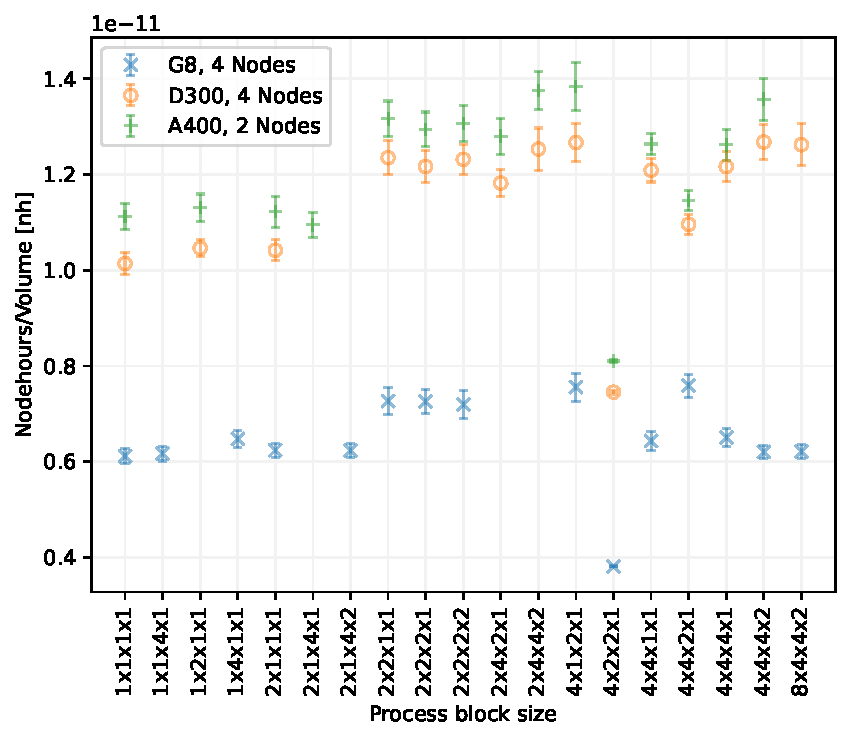
\includegraphics[width=0.6\linewidth]{\dir/img/dual_blk_numa}
%     \caption{Process block grid versus application time of the inter-grid operator moving data between the native and dual process grid. \datataking{Daint-Alps}}
%     \label{fig:dual:blk}
% \end{figure}

\tldr{dual: ranks per node}
We start investigating the effect of varying the number of ranks per node in \cref{fig:dual:tpn}.
The plot shows the number of ranks per node versus the cost in nodehours per physical lattice point for an application of the inter-grid operator while keeping the number of nodes fixed.
\num{4} ranks per node would be the case where no dual lattice is used, \ie both lattices are equal and the cost of the inter-grid operator would be \num{0} identically.
The plot shows the usual strong scaling behavior until the node memory bandwidth is saturated.
%little dependency on the number of ranks per node.
%Still the smaller the number the faster the operator.
%This is expected, because in the case of \num{8} ranks per node (we have \num{4} dual ranks per node, \ie \num{4} GPUs per node), every second rank is a dual rank.
%Meaning that only half of the global lattice has to be communicated to other processes.
%On the other side, for the case of \num{256} ranks per node, we have a dual rank every \num{64}th native rank, and thus communication of \num{63}/\num{64} of the global lattice volume.

\tldr{dual: amount of data movement}
The processes were pinned such that data exchange only happens inside a NUMA domain.
%This is only communication inside the NUMA domain.
Nevertheless, the whole field has to be moved in memory in all cases.
%, making the dependency on the ranks per node flat.
As expected, for the periodic lattice G8 compared to the the \Cstar lattice D300 (both have the same physical lattice size), we observe roughly a ratio of \num{2}.

\tldr{dual: fill node is good}
The dual lattice is primarily used when there is some non-negligible pure-MPI workload left on the CPU.
We see that the inter-grid operator performs best when filling the node with ranks.
This is fortunate because this usually holds true for the CPU workload as well.
To summarize, we can say that when working with the dual lattice, it is fine to use as many ranks per node as desired.
\begin{figure}
    \centering
    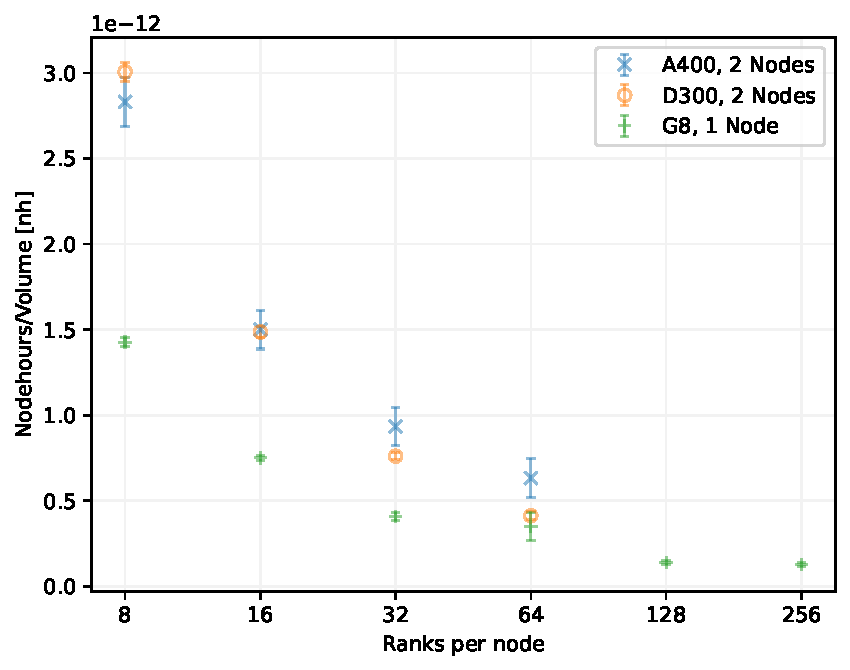
\includegraphics[width=0.6\linewidth]{\dir/img/dual_tpn_numa_shm}
    \caption{Number of native ranks per node versus application time of the inter-grid operator moving data between the native and dual process grid, keeping the number of dual ranks and nodes fixed. \datataking{Daint-Alps}}
    \label{fig:dual:tpn}
\end{figure}

\tldr{dual: strong scaling nodes}
%When choosing the ideal process block grid, which is always provided, we claimed that inter-node communication is eliminated.
We claimed in \cref{sec:interface:openqxd:dual} that inter-node communication is eliminated.
This is shown in \cref{fig:dual:nodes}.
We observe embarrassingly parallel behavior with respect to the number of nodes, even when going up to \num{128} nodes (\num{512} GPUs) on the smallest lattice making the inter-grid operator strong scaling ideal.
The base-case for the \Cstar lattices is \num{2} nodes (\num{8} GPUs) because of an implementation restriction\footnote{The current implementation demands a process grid length of at least 2 in every direction that is a spatial C$^\star$-direction. With 3 C$^\star$ directions this gives a minimum of 8 processes, \ie 8 GPUs unless one uses MPS or MIG. MPS gives a severe performance degradation of the GPU part, and MIG is not available on request on \emph{Daint-Alps}.}.
%This behavior implies that if the inter-grid operator is too expensive, one can always make its contribution negligible by increasing the number of nodes.
\begin{figure}
    \centering
    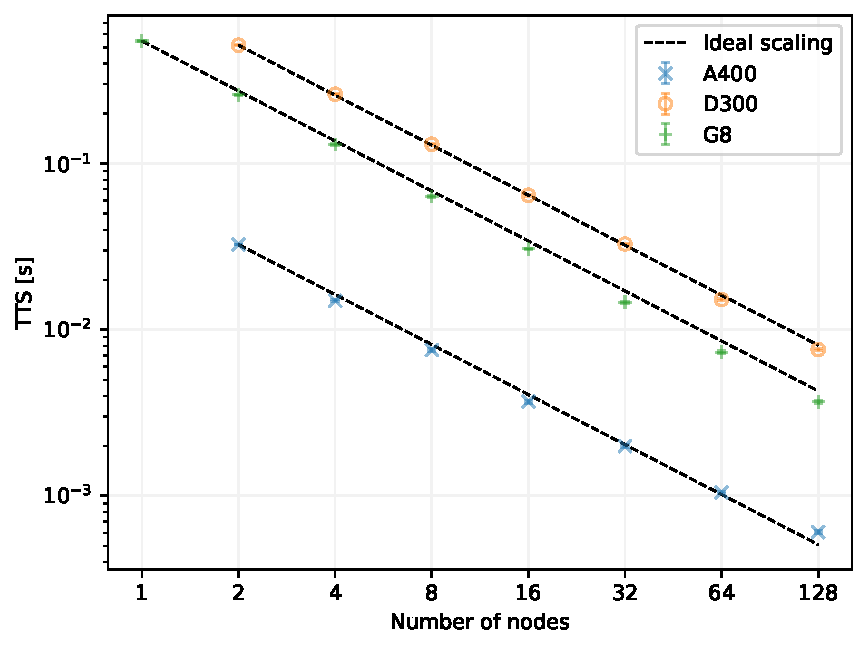
\includegraphics[width=0.6\linewidth]{\dir/img/dual_nodes}
    \caption{Strong scaling of inter-grid operator. Number of nodes versus application time of the inter-grid operator, keeping the number of native and dual ranks per node fixed. \datataking{Daint-Alps}}
    \label{fig:dual:nodes}
\end{figure}

\tldr{dual: contribution negligible}
Finally, we discuss the contribution of the inter-grid operator to a solve of the Dirac equation using a multigrid solver -- a production example of the dual grid in action is given in \cref{fig:dual:bar}.
The plot shows five contributions; moving the source vector from the native to the dual lattice (blue) and subsequently to the GPU (green), solving the linear system of equations on the GPU (purple), moving the solution vector from the GPU back to the dual lattice (red) and subsequently to the native lattice (yellow).
%First, as expected the D2H/H2D transfers and the inter-grid data movement operators perform very similar, since both move about the same amount of data in memory and both are bound by memory bandwidth.
We see that the inter-grid contribution decreases as one increases the node count, same holds true for CPU-GPU transfers.
This is expected, since both kernels involve no communication.
The only contribution that does not strong scale perfectly -- the solver itself as we will see later -- increases its contribution when increasing the number of nodes.
However, we observe that the inter-grid operator contributes negligibly to the overall solve.
\begin{figure}
    \centering
    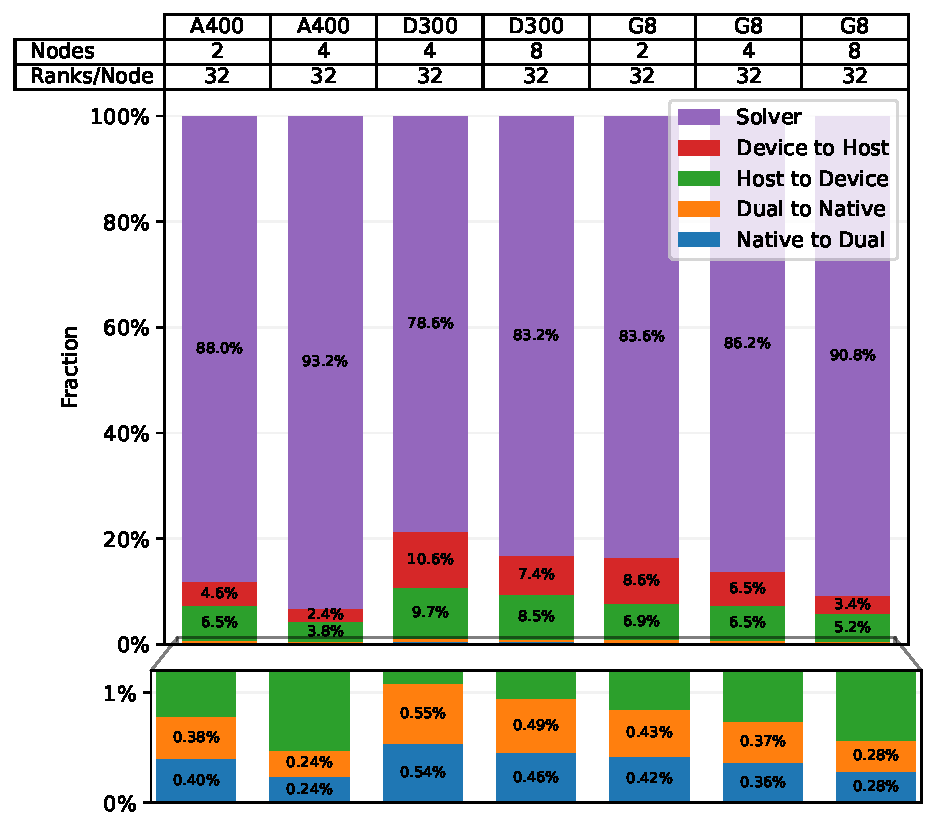
\includegraphics[width=0.8\linewidth]{\dir/img/dual_bar_numa_shm}
    \caption{Contribution of data movement kernels to the solver. The plot shows different lattices and setups specified on the x-axis. Blue and yellow indicate the inter-grid data movement operator between the native and dual process grids, whereas green and red indicate the CPU-GPU data transfer and reordering procedure. Finally purple shows the contribution of the actual multigrid Krylov solver on the GPU. The contribution of the inter-grid operator is negligible in all cases as can be seen in the inset. \datataking{Daint-Alps}}
    \label{fig:dual:bar}
\end{figure}

\tldr{dual: numa placement: 10-20 percent additional speedup}
Regarding the dual lattice, we ensured that native and dual processes corresponding to the same local lattices were in the same NUMA domain to prevent communication from one NUMA domain to another further optimizing its performance.
Due to the difference in processes numbering in periodic and \Cstar cases, see \cref{eq:dual:rank:condition:periodic,eq:dual:rank:condition:cstar}, the CPU-binding has to be different as well.
To illustrate this, we show an explicit example of the pinning and core distribution for a run with a single GH200 node and \num{32} rank per node in \cref{tab:perf:numa:periodic,tab:perf:numa:cstar} for periodic and \Cstar boundary conditions, respectively.
The additional effect on performance of correct NUMA placement was in the regime of \SIrange{10}{20}{\percent}.

\begin{table}[h]
\centering
\begin{tabular}{cccccccc}
\multicolumn{4}{c}{Native} & \multicolumn{4}{c}{Dual} \\
\cmidrule(lr){1-4}
\cmidrule(lr){5-8} 
\makecell{MPI\\rank} &
\makecell{Core\\ID} &
\makecell{NUMA\\domain} &
\makecell{CPU\\ID} &
\makecell{MPI\\rank} &
\makecell{Core\\ID} &
\makecell{NUMA\\domain} &
\makecell{GPU\\ID} \\
\cmidrule(lr){1-4}
\cmidrule(lr){5-8} 
0-7   & 0-7     & 0 & 0 & 0  & 0   & 0 & 0 \\
8-15  & 72-79   & 1 & 1 & 8  & 72  & 1 & 1 \\
16-23 & 144-151 & 2 & 2 & 16 & 144 & 2 & 2 \\
24-31 & 216-223 & 3 & 3 & 24 & 216 & 3 & 3 \\
\end{tabular}
\caption{Example of NUMA process placement to core IDs with periodic boundaries. With \num{32} tasks per node, we divide them into \num{8} tasks per NUMA domain associated to one CPU, filling only \num{8} from the available \num{72} cores. The dual MPI rank is calculated using \cref{eq:dual:rank:condition:periodic} and should be in the same NUMA domain. The GPUs are in NUMA domains \num{4},\num{12},\num{20} and \num{28} but also affine to \num{0}, \num{1}, \num{2} and \num{3}, respectively.}
\label{tab:perf:numa:periodic}
\end{table}

\begin{table}[h]
\centering
\begin{tabular}{cccccccc}
\multicolumn{4}{c}{Native} & \multicolumn{4}{c}{Dual} \\
\cmidrule(lr){1-4}
\cmidrule(lr){5-8} 
\makecell{MPI\\rank} &
\makecell{Core\\ID} &
\makecell{NUMA\\domain} &
\makecell{CPU\\ID} &
\makecell{MPI\\rank} &
\makecell{Core\\ID} &
\makecell{NUMA\\domain} &
\makecell{GPU\\ID} \\
\cmidrule(lr){1-4}
\cmidrule(lr){5-8} 
$0,2, \ldots, 14$   & 0-7     & 0 & 0 & 0  & 0   & 0 & 0 \\
$1,3, \ldots , 15$  & 72-79   & 1 & 1 & 1  & 72  & 1 & 1 \\
$16,18, \ldots, 30$ & 144-151 & 2 & 2 & 16 & 144 & 2 & 2 \\
$17,19, \ldots, 31$ & 216-223 & 3 & 3 & 17 & 216 & 3 & 3 \\
\end{tabular}
\caption{Example of NUMA process placement to core IDs with \num{32} tasks per node and \Cstar boundaries. For detail see \cref{tab:perf:numa:periodic}.}
\label{tab:perf:numa:cstar}
\end{table}
% 0,72,1,73,2,74,3,75,4,76,5,77,6,78,7,79,144,216,145,217,146,218,147,219,148,220,149,221,150,222,151,223

\tldr{dual: summary}
We investigated the behavior and contributions of the dual process grid.
Its contribution was negligible in all cases and can even be pushed down further by increasing the number of nodes due to its perfect strong scaling.
However, the solver algorithm does not strong scale perfectly as we will see later.
This trade-off has to be taken into account when considering the setup.
%However, the trade-off that the solver itself does not strong scale perfectly has to be taken into account when considering the node count.
As usual in HPC, the best performing setup is a compromise between multiple competing motives.
The largest contribution should be considered primarily.

\section{The asynchronous solver}
\label{sec:perf:solver:async}

\tldr{async: CPU kernel description}
Heterogeneous computing can be achieved by overlapping expensive solves on the GPU with some independent work on the CPU by using the asynchronous solver interface introduced in \cref{sec:interface:solver:async,sec:develop:async:way}.
The performance of different kernels on the CPU overlapping with solves on the GPU were assessed in \cref{fig:async:F7:leo:bar}.
%The CPU kernels are described as follows:
Kernels on the CPU are described as follows:
\begin{enumerate}[label=\alph*)]
    \item \emph{sleep()}: This kernel is trivial and serves as a baseline. While the GPU performs the solve, the CPU repeatedly calls \code{nanosleep()} for about the same amount of time.
    \item \emph{I/O}: A pure I/O kernel performing a read-in of a large amount of data located on a scratch filesystem with very few MPI calls of little data amounts.
    \item \emph{I/O+MPI}: A kernel performing the same read-in as before, but additionally the data is scattered among all ranks via MPI.
    \item \emph{Dirac operator}: Repeated applications of the Dirac stencil, a memory bandwidth bound operation including halo exchange and barriers.
    \item \emph{MPI\_Allreduce()}: Repeated applications of \code{MPI\_Allreduce()} to comparably small amounts of data. This is a pure MPI kernel doing only communication.
    \item \emph{Memory}: A pure local memory traffic producing kernel without any communication, accessing rank-local data repeatedly.
\end{enumerate}

\tldr{async: leonardo, contributions}
In \cref{fig:async:F7:leo:bar}, we observe clear speedups of the heterogeneous case compared to the serial execution model.
Slight performance degradation only occurs in kernels heavily utilizing MPI.
Furthermore, the performance of the solve on the GPU is only negligibly affected by the concurrent work done on the CPU.
\begin{figure}
    \centering
    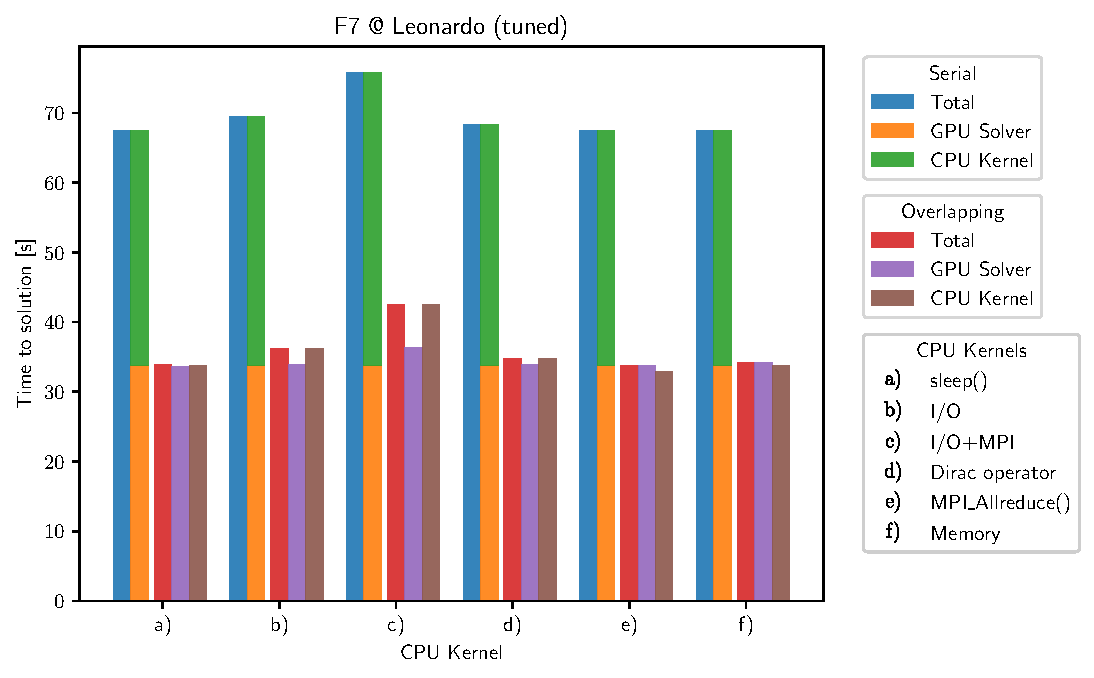
\includegraphics[width=\linewidth]{\dir/img/async_leo_F7.A}
    \caption{Contributions from different kernels a) to f) on the CPU to a Krylov solve on the GPU. Blue, yellow and green show the serial pipeline (see \cref{fig:develop:serial,lst:develop:serial}), whereas red, purple and brown show the overlapping pipeline (see \cref{fig:develop:pipelining,lst:develop:pipelining}) averaged over \num{10} solves. \datataking{Leonardo Booster}}
    \label{fig:async:F7:leo:bar}
\end{figure}

\tldr{async: leonardo, speedups}
\Cref{fig:async:F7:leo:speedup} shows the speedup of the overlapping case over the serial workload.
The GPU solver as well as the CPU kernels are barely affected by overlapping, resulting in a total speedup close to the analytic limit of \num{2} for all kernels.
This means we can successfully hide the entire CPU or GPU work by instantiating a pipelined execution model and fully utilize all available resources in a node.
\begin{figure}
\centering
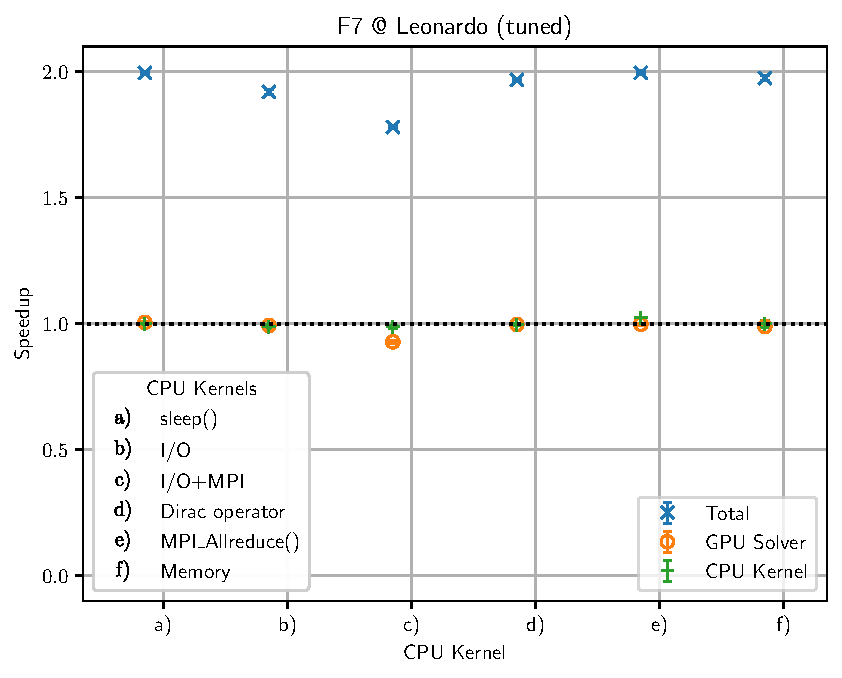
\includegraphics[width=0.6\linewidth]{\dir/img/async_leo_F7.B}
\caption{
Absolute speedup of the heterogeneous versus the serial execution model averaged over \num{10} solves.
A speedup of \num{2} is the analytical maximum.
%A data point above \num{1} results in a speedup, whereas a data point below \num{1} results in a slowdown.
The effect of overlapping for the GPU solve as well as the individual kernels are indicated by yellow and green, whereas the blue shows the net speedup when overlapping.
\datataking{Leonardo Booster}
% \worktodo{add arrows speedup/degradation, add errorbars}
}
\label{fig:async:F7:leo:speedup}
\end{figure}

\tldr{async: daint, contributions}
The data for the heterogeneous solver was taken on \emph{Leonardo Booster}.
It is worth looking at the same plot for a GH200 node at \emph{Daint-Alps}, see \cref{fig:async:F7:daint:bar}.
The data shows a completely different picture: it is not worth doing entirely.
On the contrary; performance is even degraded compared to the serial case.
This originates from the fact that currently the power module of the GH200 node at CSCS is capped at around \SI{650}{\watt} and the CPU will always draw as much power from it as it can, letting the GPU starve.
The two devices compete for energy.
On such a machine, a serial execution model performs better, because when the CPU draws power, the GPU is idle and vice versa.
As backed by the data in the plot, it is currently\footnote{The problem is known by CSCS, NVIDIA and HPE.} not a good idea to overlap CPU and GPU calculations on the GH200 node.
\begin{figure}
    \centering
    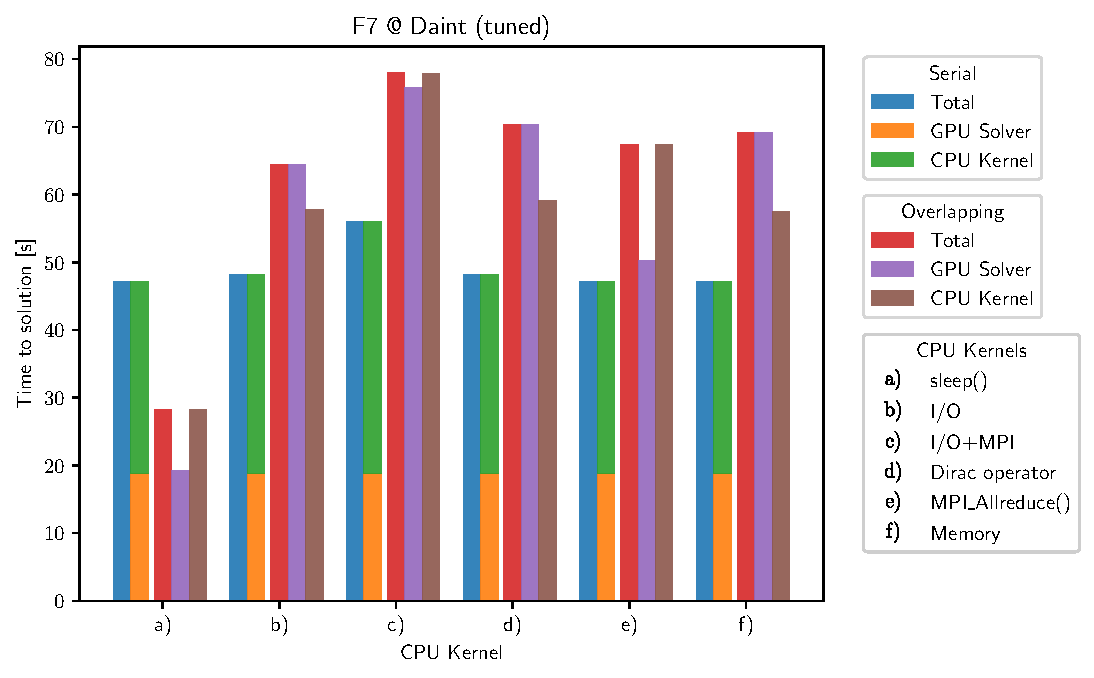
\includegraphics[width=\linewidth]{\dir/img/async_daint_alps_F7.A}
    \caption{Contributions from different kernels a) to f) on the CPU to a Krylov solve on the GPU. Blue, yellow and green show the serial pipeline (see \cref{fig:develop:serial,lst:develop:serial}), whereas red, purple and brown show the overlapping pipeline (see \cref{fig:develop:pipelining,lst:develop:pipelining}) averaged over \num{10} solves. \datataking{Daint-Alps}}
    \label{fig:async:F7:daint:bar}
\end{figure}

\section{The multiple right-hand sides solver}
\label{sec:perf:solver:mrhs}

\tldr{mrhs: daint speedup data}
The multiple right-hand sides solver interface is discussed in \cref{sec:interface:solver:mrhs} and can be accessed as described in \cref{sec:develop:mrhs:way}.
\Cref{fig:mrhs:tts} shows its speedup versus the number of right-hand sides. %, where all right-hand sides are solved simultaneously.
The base case is a single right-hand side.
The theoretical maximal speedup\footnote{
This number is obtained by considering a performance model as
\begin{align}
\text{cost}(1)      &= \mem(D) + 2 x \cdot \mem(\psi) \;,    &\text{single RHS} \,, \\
\text{cost}(\infty) &= 2 x \cdot \mem(\psi) \;,              &\text{for } \Nrhs \to \infty  \,,
\end{align}
for the cost of an application of the Wilson-Clover Dirac operator, where $\mem(A)$ denotes the memory traffic of the object $A$.
Naively $x=8$ for fetching \num{8} neighboring points and $x=1$ for perfect caching.
The reality is in between.
Thus, using $\mem(D) = 6 \cdot \mem(\psi)$, the ratio of these two $\frac{\text{cost}(1)}{\text{cost}(\infty)} = \frac{x+3}{x} \in \left[ 1.375, 4 \right]$.
} is around 1.375-4 .
On the small lattice A400 we reach a higher speedup as on the large lattice D300.
This is due to the fact that the increase in data locality and parallelism has a higher impact on small problems which are already in the bad strong scaling region as opposed to large ones.
However, the speedup directly translates to cost efficiency.
\begin{figure}
    \centering
    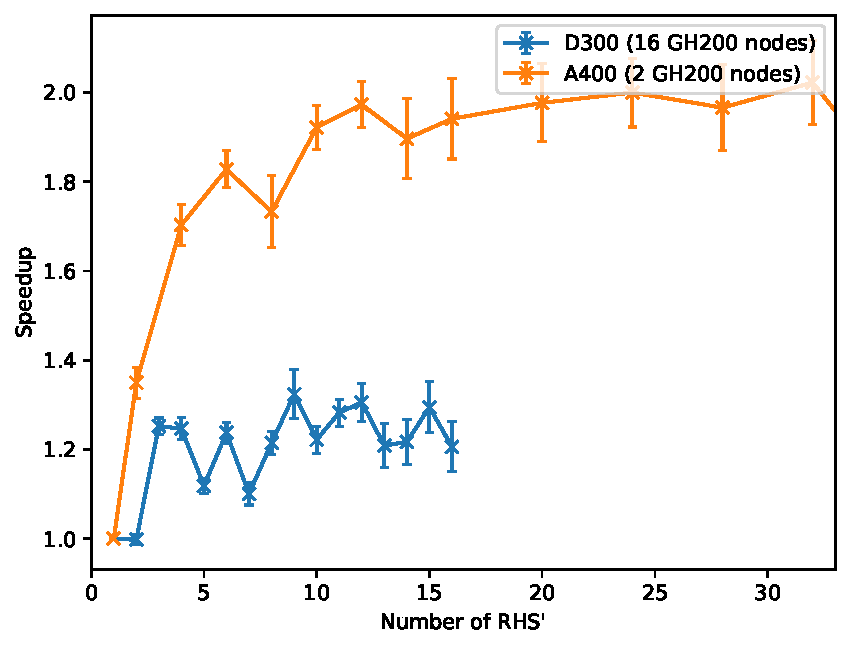
\includegraphics[width=0.7\linewidth]{\dir/img/mrhs_tts}
    \caption{Number of right-hand sides versus speedup compared to a single right-hand side. For small problems, a twofold speedup is reached. \datataking{Daint-Alps}}
    \label{fig:mrhs:tts}
\end{figure}

\tldr{mrhs: daint energy consumption}
It is worth to study the impact on energy consumption in \cref{fig:mrhs:energy}.
%It is worth studying the cost in terms of energy consumption of the solver when solving multiple RHSs in \cref{fig:mrhs:energy}.
The better temporal data locality and larger local problem size allows us to come closer to saturating the GPU.
As we increase the number of RHSs, the energy required per solve decreases, whereas the power drawn from the power module increases.
Saturation can be observed at about \numrange{12}{16} RHSs.
This is a clear indication that the lattice considered is too small for \num{2} Quad GH200 nodes, not exposing enough parallelizability.
On the other hand, solving \num{16} or more RHSs at the same time exposes substantially more parallelizability to the GPU and is able to saturate the \num{2} nodes.
Even more importantly the energy cost per solve decreases by a factor of about \num{1.6}.
\begin{figure}
    \centering
    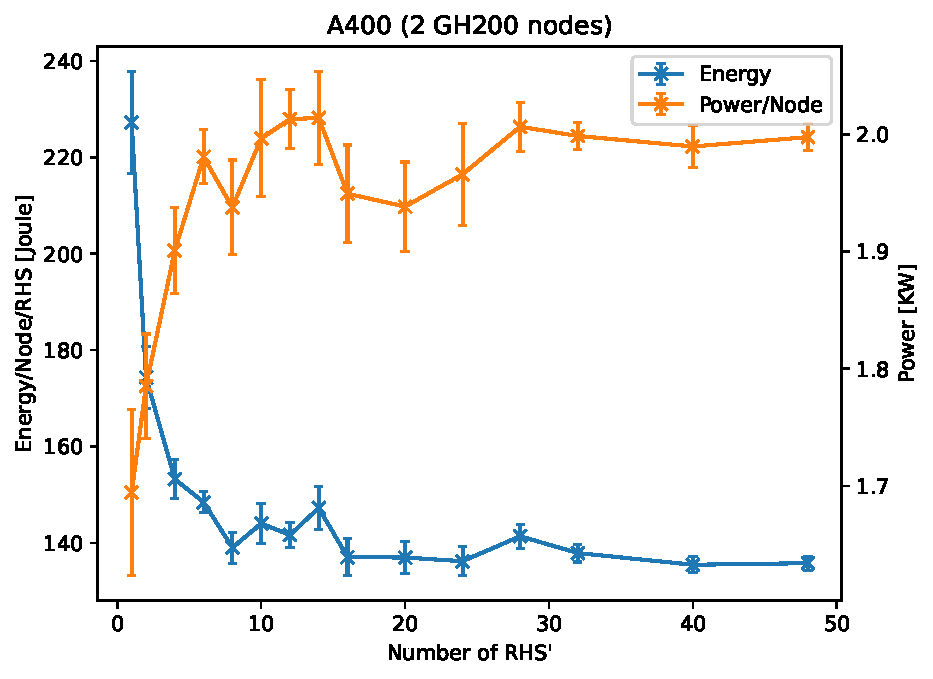
\includegraphics[width=0.7\linewidth]{\dir/img/mrhs_energy}
    \caption{Number of right-hand sides versus energy consumption per RHS per node (blue) and versus power drawn from the power module per node (yellow) of the A400 lattice running on 2 nodes. Increasing the number of RHSs saturates the nodes. \datataking{Daint-Alps}}
    \label{fig:mrhs:energy}
\end{figure}

\section{Dirac operator}
\label{sec:perf:dop}

\tldr{Dop important kernel in solvers}
One of the most important kernels of every lattice application is the Dirac operator, \cref{eq:Dw:QCD+QED}.
It is crucial to have an efficient implementation of the Dirac stencil, since iterative Krylov solvers themselves call the operator once or twice in every iteration.
We are interested in the pure nearest-neighbor stencil as it appears in solver algorithms.
Thus, we assume the field to already reside in HBM memory on the GPU and the following plots will neither include H2D nor D2H transfers.

\tldr{Dop: strong scaling daint}
\Cref{fig:daint:alps:dw:strong} shows strong scaling of the GPU implementation of the Dirac operator.
We focused on a periodic and a \Cstar lattice with the same global physical lattice extents of $L_0 \times L^{3} = 128 \times 64^{3}$.
The time taken was averaged over \num{10000} invocations to the operator and at least \num{5} independent runs were conducted for every data point.
We observe decent strong scaling.
For this lattice size on a GPU, it is expected that for \num{64} to \num{256} nodes (\num{256} to \num{1024} GPUs) the scaling is far from ideal.
One reason is a too small local problem size to saturate the high parallelizability of the H100.
For comparison, the local lattice size for the \num{256} node case is $16^{4}$ resulting in a local vector size of about \SI{12.58}{MB}.
One H100 has \num{132} streaming multiprocessors (SMs), \num{64} warps per SM with a warp size of \num{32}.
Therefore, the $16^{4}$ local lattice, with its \num{65536} lattice points, is distributed to \num{270336} available CUDA threads on a single H100.
Even the smaller \num{64} node case with \num{262144} local lattice points is barely able to saturate the machine.
\begin{figure}
    \centering
    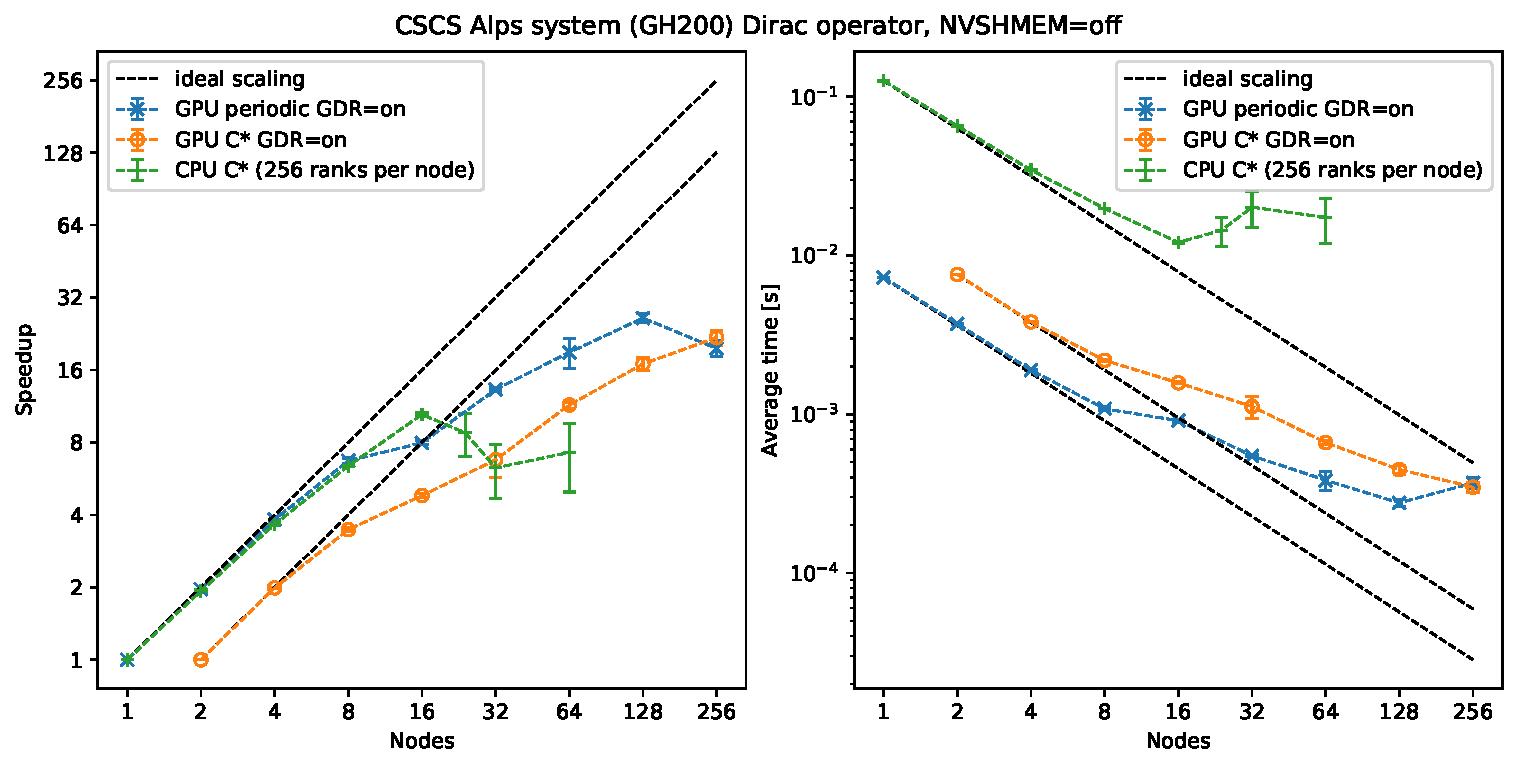
\includegraphics[width=0.9\linewidth]{\dir/img/daint_alps_dw_strong}
    \caption{Strong scaling of Dirac stencil (left panel) and average time for one application (right panel). The operator was applied \num{10000} times and the average was taken. The base case for the \Cstar lattice is two nodes for implementation restrictions. The physical global lattice size was $T \times L^{3} = 128 \times 64^{3}$ for all runs. Every data point consists of at least \num{5} independent runs. \datataking{Daint-Alps}}
    \label{fig:daint:alps:dw:strong}
\end{figure}

\tldr{Dop: weak scaling daint}
Since the performance of the operator only depends on the problem size and boundary conditions but not on physics parameters, we can easily run it on synthetic data to obtain a weak scaling plot as in \cref{fig:daint:alps:dw:weak}.
In the weak scaling study, the physical local lattice size is kept constant.
This is $64 \times 32 \times 64 \times 64$ for the periodic lattice and $128 \times 32 \times 64 \times 32$ for the \Cstar lattice.
These numbers were chosen such that both lattices show the exact same global lattice extents for the \num{2} node case and onward.
Additionally, the number of local lattice points (about \SI{8}{m} for periodic and double that for \Cstar) is significantly larger than the number of CUDA threads in the H100.
As expected, since the local problem size stays large we observe solid weak scaling of the Dirac stencil, with still \SI{80}{\percent} efficiency at \num{1024} GPUs.
The good weak scaling makes the software stack ready for larger problem sizes.
\begin{figure}
    \centering
    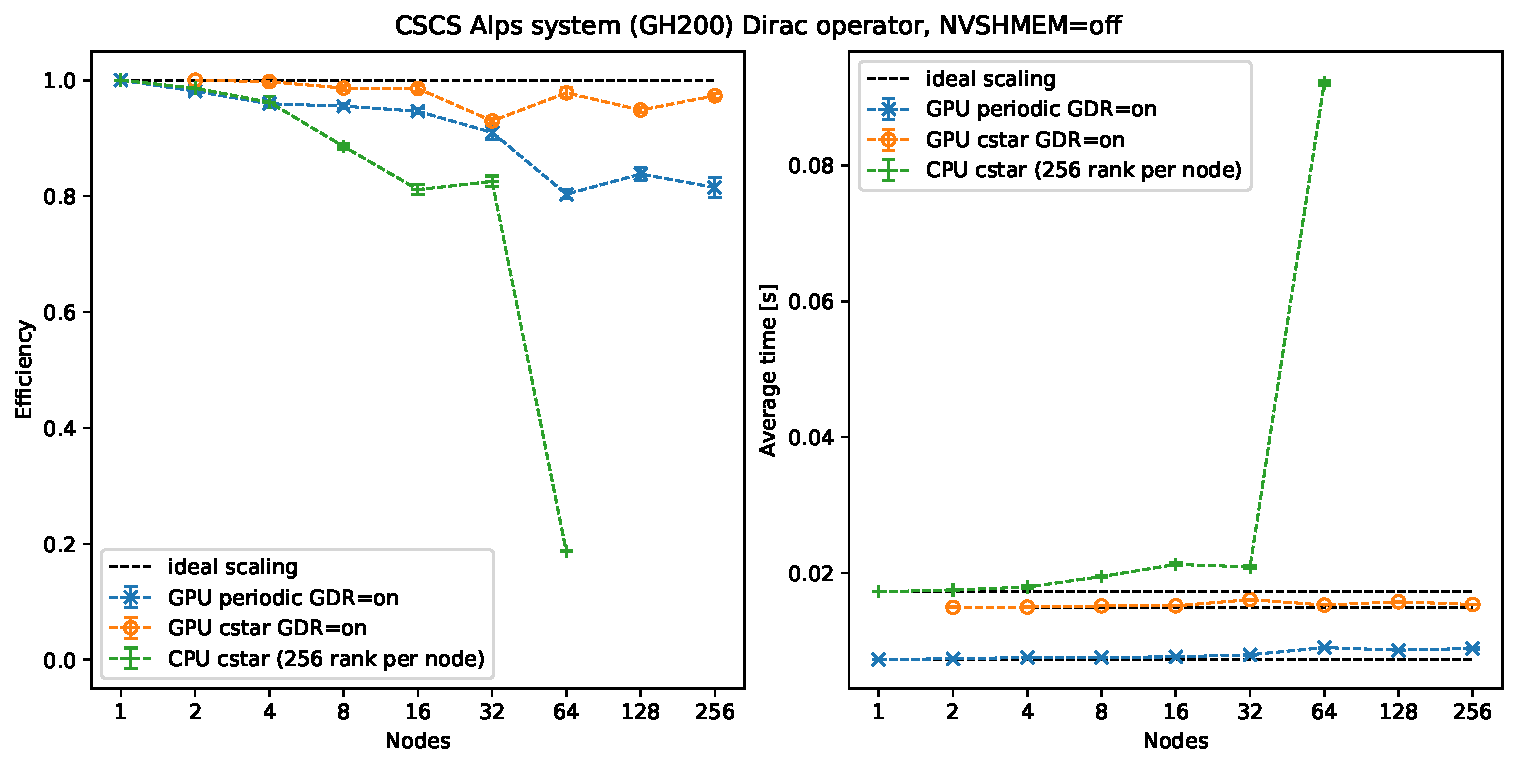
\includegraphics[width=0.9\linewidth]{\dir/img/daint_alps_dw_weak}
    \caption{Weak scaling of Dirac stencil (left panel) and average time for one application (right panel). The operator was applied \num{10000} times and the average was taken. The base case for the \Cstar lattice is two nodes for implementation restrictions. The physical local lattice size was $64 \times 32 \times 64 \times 64$ and $128 \times 32 \times 64 \times 32$ for the periodic and \Cstar lattice, respectively. Every data point consists of at least \num{5} independent runs. \datataking{Daint-Alps}}
    \label{fig:daint:alps:dw:weak}
\end{figure}

\tldr{Dop: no nvshmem}
For the strong and weak scaling runs, we did not utilize NVIDIA shared memory (NVSHMEM) because it was not yet available on the cluster.
NVSHMEM is NVIDIAs implementation of the OpenSHMEM standard~\cite{online:openshmem}, a parallel programming model and library designed to facilitate efficient data sharing and communication between GPUs, both within a single node and across multiple nodes.
NVIDIA promises less overhead resulting in more efficient strong scaling when using NVSHMEM~\cite{online:nvshmem}.
However, the Cray MPI implementation was CUDA-aware, Peer to Peer access (P2P) from GPUs within the same node was utilized, and GPU-direct RDMA (GDR) was enabled to further remedy bad strong scaling behavior.
Nevertheless, the error bars might be slightly underestimated because of temporal correlations among runs, especially for runs with high node counts.

%\worktodo{say something about nvshmem, gives better strong scaling ...}
%\worktodo{say something about GDR}
%\worktodo{weird bump in weak scaling, probably due to network contention on the cluster}
%\worktodo{strong/weak scaling plots, maybe multiple independent runs? not 5 on the same setup?}
%\worktodo{outlier treatment: no treatment}
%\worktodo{error underestimated, because temporal correlation between runs, they might get the same node setup}

\section{Solver}
\label{sec:perf:solver}

\tldr{solver intro}
As opposed to the Dirac operator, the convergence rate of a Krylov solve \emph{does} depend on the physics parameters and the background gauge field non-trivially.
Therefore, we cannot present a thorough weak scaling study for the solver.
For the discussion of strong scaling of the solver that follows, we took representative gauge field configurations and fixed physics parameters.

\tldr{solver: strong scaling on daint}
\Cref{fig:daint:alps:inv:strong} shows strong scaling of a production multigrid solver on a periodic and a \Cstar lattice.
The relative residual is chosen to be $10^{-12}$ for all solves.
We see very poor strong scaling above \numrange{16}{32} nodes.
This is expected because unfortunately multigrid preconditioning inherently possesses bad strong scaling behavior.
This is due to the fact that multigrid coarsens the lattice into a smaller lattice with significantly fewer degrees of freedom and solves the Dirac equation on the coarse lattice in every iteration step.
The repeated coarse lattice solves, which dominate the runtime, are by far not able to saturate the GPU especially for high node counts.
Clearly, an unpreconditioned solver would show better strong scaling that is comparable to the Dirac operator itself (see \cref{fig:daint:alps:dw:strong}), but on ill-conditioned systems such a solver would take thousands of iteration steps or never converge at all.
Multigrid is the state-of-the-art production solver for ill-conditioned systems in the field.
Its time to solution is paramount with the trade-off of bad strong scaling.

%It is a periodic extension of D300 respecting global boundary conditions.
%Its scaling is good up to \num{512} GPUs.
For this reason, the plot shows a third (somewhat artificial) lattice D300x16.
This lattice consists of periodically extended copies of D300 in all \num{4} spacetime directions by a factor of \num{2} respecting global boundary conditions, \ie, \num{16} times larger than the original D300.
Such a lattice belongs to the largest ones appearing in the field (sometimes called monster lattice).
D300x16 has physical lattice extents $L_0 \times L^{3} = 256 \times 128^{3}$.
The fact that this lattice scales well up to \num{512} GPUs indicates that the code is ready for substantially larger problem sizes.

\begin{figure}
\centering
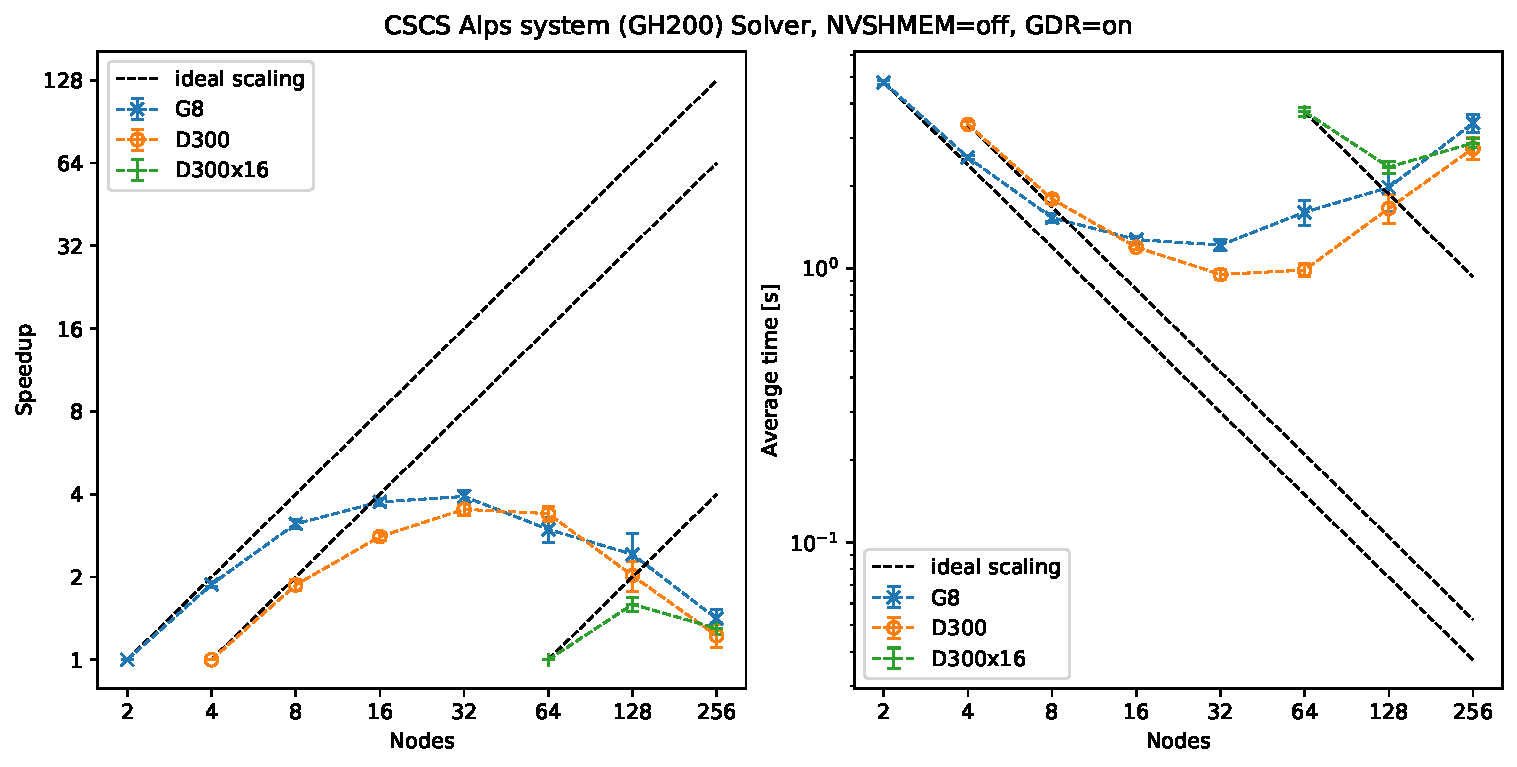
\includegraphics[width=0.9\linewidth]{\dir/img/daint_alps_inv_strong}
\caption{
Strong scaling of a multigrid solver (left panel) and average time to solution for one solve (right panel).
The base cases were chosen to be the smallest node count for the computation to fit in GPU memory.
\datataking{Daint-Alps}}
\label{fig:daint:alps:inv:strong}
\end{figure}

% \tldr{solver: scaling with mrhs (weak) on daint}
% The discussion in the previous paragraph suggests that if we saturate the GPU by exposing more parallelizability on the lattices which are too small, we should observe better scaling behavior.
% This can be achieved by solving for multiple right-hand sides at the same time.
% \Cref{fig:daint:alps:inv:weak:mrhs} shows a variant of a weak scaling study where not the local problem size was held constant but the computational work per node in terms of RHSs.
% As the number of nodes increases the number of RHSs increases proportionally, thus, the local workload stays constant as opposed to the local lattice size.
% The plot shows some interesting features worth mentioning.
% The super-linear efficiency for the small node counts comes from the better data locality and increased arithmetic intensity when processing more than one RHS at the same time.
% The improvement diminishes again quickly, since even though the local size of the RHSs stays constant, the local \emph{problem} size -- and by this the local operator size in memory -- decreases inversely proportional to the node count.
% Processing multiple RHS turns matrix-vector into matrix-matrix multiplications, increasing the arithmetic intensity.
% In the plot, the matrix representing the RHSs stays constant in total size but its dimensions change, whereas the operator matrix size decreases.
% There are numerous competing concepts affecting the overall performance in this scenario.
% As the number of RHS increases, we expect better temporal data locality and cache reuse until batch sizes exceed cache or shared memory capacity clearly visible in the plot.
% Since the amount of local variables scales linear in the number of RHSs, we expect variables to the moved to slower memory resulting in register spilling~\cite{CHAITIN198147} as the number RHSs increases.
% Finally, as the RHS matrix changes shape stride access pattern can cause data in cache to repeatedly being evicted resulting in cache thrashing~\cite{10.1145/1476589.1476705}.
%However for intermediate node counts, we see good scaling behavior.
% \begin{figure}
% \centering
% 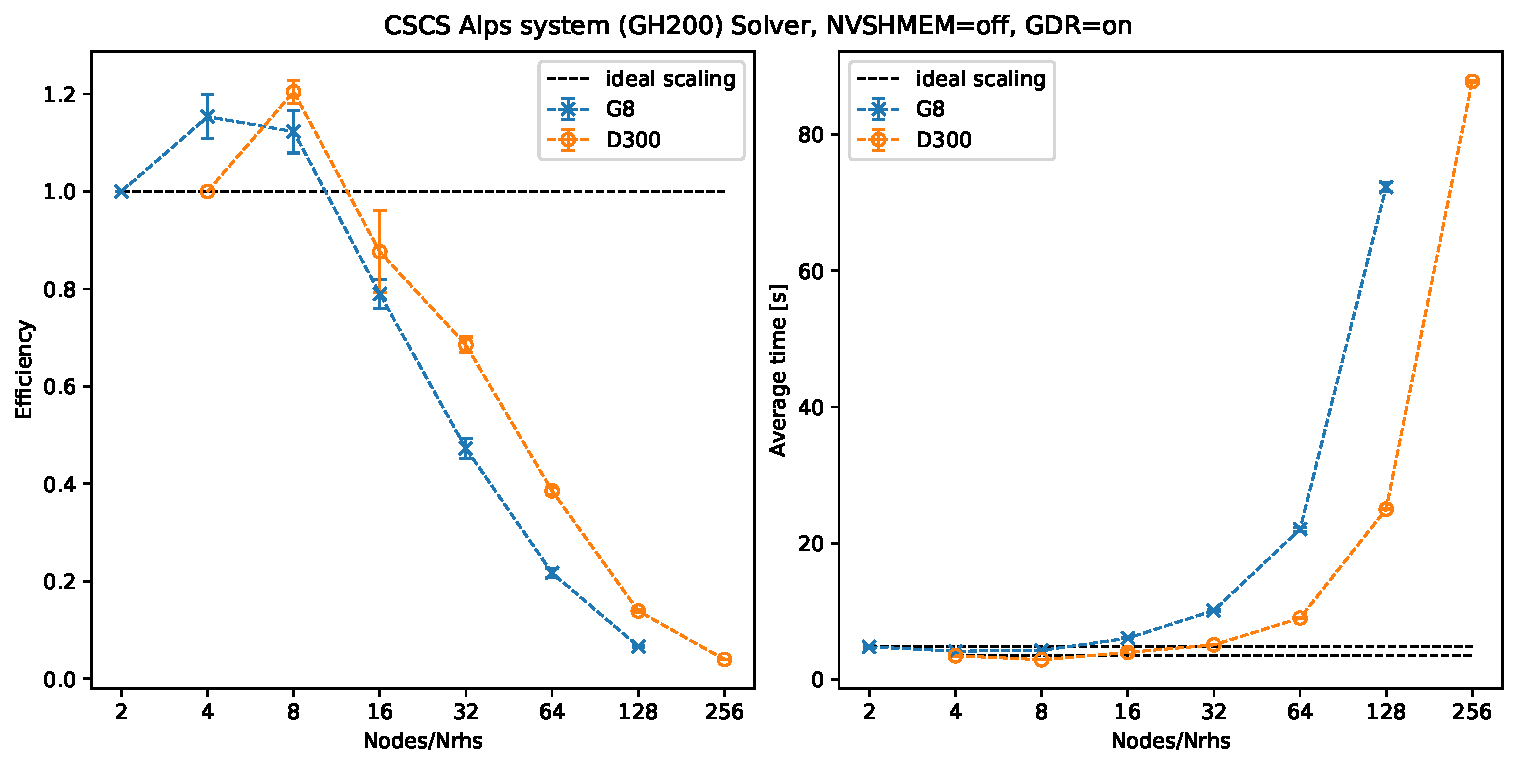
\includegraphics[width=0.9\linewidth]{\dir/img/daint_alps_inv_weak_mrhs}
% \caption{
% Variant of weak scaling of a multigrid solver w.r.t. number of RHSs (left panel) and average time to solution for all RHSs (right panel).
% The base cases were chosen to be the smallest node count for the computation to fit in GPU memory.
% \datataking{Daint-Alps}
% \worktodo{remove red from plot}
% }
% \label{fig:daint:alps:inv:weak:mrhs}
% \end{figure}


\tldr{solver: scaling with mrhs (strong) on daint}
The discussion in the previous paragraph suggests that if we saturate the GPU by exposing more parallelizability on the lattices which are too small, we should observe better scaling behavior.
This can be achieved by solving for multiple right-hand sides at the same time.

\Cref{fig:daint:alps:inv:strong:mrhs} shows a variant of a strong scaling study where as the node count is increased the number of RHSs increases proportionally.
% As the number of nodes increases the number of RHSs increases proportionally, thus, the local workload stays constant as opposed to the local lattice size.
The plot shows some interesting features worth mentioning.
The super-linear efficiency for the small node counts comes from the better data locality and increased arithmetic intensity when processing more than one RHS at the same time.
The improvement diminishes again quickly, since even though the local size of the RHSs stays constant, the local \emph{problem} size -- and by this the local operator size in memory -- decreases inversely proportional to the node count.

Processing multiple RHS turns matrix-vector into matrix-matrix multiplications, increasing the arithmetic intensity.
In the plot, the matrix representing the RHSs stays constant in total memory size but its dimensions change, whereas the operator matrix size decreases.

There are numerous competing concepts affecting the overall performance in this scenario.
As the number of RHS increases, we expect better temporal data locality and cache reuse until batch sizes exceed cache or shared memory capacity clearly visible in the plot.
Since the amount of local variables scales linear in the number of RHSs, we expect variables to the moved to slower memory resulting in register spilling~\cite{CHAITIN198147} as the number RHSs increases.
Finally, as the RHS matrix changes shape stride access pattern can cause data in cache to repeatedly being evicted resulting in cache thrashing~\cite{10.1145/1476589.1476705}.

Nevertheless the strong scaling improves.
The degradation at about \num{64} nodes in \cref{fig:daint:alps:inv:strong:mrhs}, could be lifted further by increasing the number of RHSs as the local problem size still diminishes too quickly.
\begin{figure}
\centering
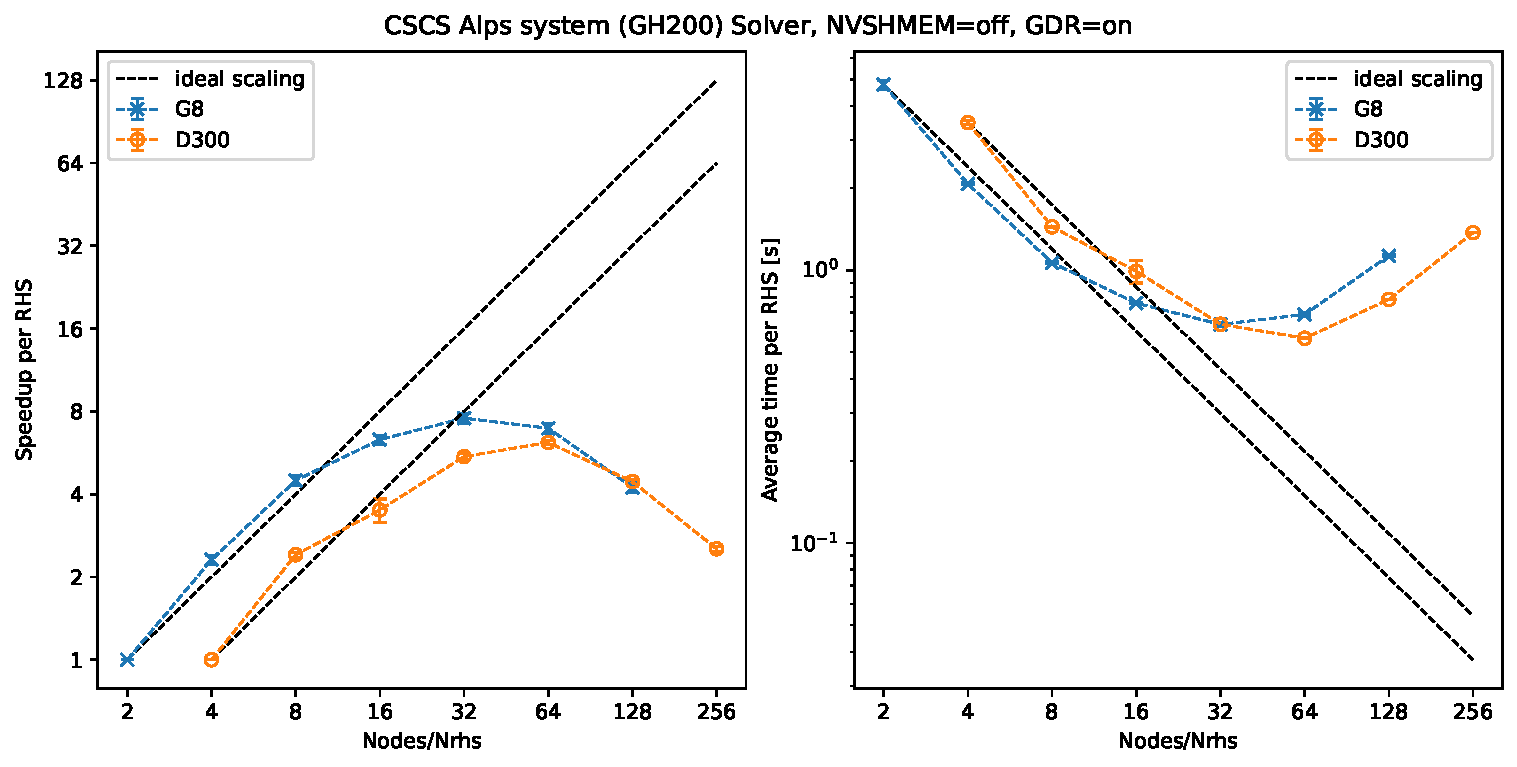
\includegraphics[width=0.9\linewidth]{\dir/img/daint_alps_inv_strong_mrhs}
\caption{
Strong scaling of a multigrid solver w.r.t. number of RHSs and nodes (left panel) and average time to solution for all RHSs (right panel).
The base cases were chosen to be the smallest node count for the computation to fit in GPU memory.
\datataking{Daint-Alps}
}
\label{fig:daint:alps:inv:strong:mrhs}
\end{figure}

\section{Summary}
\label{sec:perf:summary}

\tldr{performance data conclusion}
Wrapping up the performance chapter, we conclude that on a cluster with GH200 nodes with lattices currently accessible to us, we can utilize the resources of the node efficiently.
However, performing runs with more than \num{32} GH200 nodes is not advisable because then we are clearly in the bad strong scaling region unless we study larger lattices as the ones considered or increase the number of RHSs substantially.
In a field where the total problem size naturally grows with the available compute power, good weak scaling makes our software stack future-proof.
The fact that the largest lattice considered strong scales up to \num{512} GPUs indicates that the code is ready for the exascale.

%On the other side, evaluating observables usually consists of computations on $\bigO(1000)$ independent gauge field configurations.
%Solving the Dirac equation on all configs of an ensemble can easily be done embarrassingly parallel with one job of size \numrange{8}{16} nodes per config and a RHS batch size of \numrange{4}{32}.

Computations on the CPU can efficiently be overlapped with concurrent solves on the GPU, if power supply of the machine allows it as proven on \emph{Leonardo Booster}.
Finally, for maximizing node utilization of reminiscent CPU workloads, it can conveniently be scaled out within the node by using the dual process grid adding negligible performance overhead.

The inherent challenging strong scaling of multigrid is not a big problem for multiple reasons.
First, we now have many tools available to mitigate it, such as overlapping multigrid solves with computations on the CPU or solving an array of RHSs in one batch.
Second, in reality the only relevant metric usually boils down to time or energy to solution.


The data still shows some non-negligible contributions of H2D and D2H transfers (red and green in \cref{fig:dual:bar}).
In future developments, the H2D transfers could be eliminated to a large extent by setting up the source vector directly on the GPU, especially when dealing with random or point sources.
Instead of handing over the field data, we hand over a description of the field instead.
Field transfers in general can be reduced by employing a memory management system keeping track of field status.
A system minimizing CPU-GPU traffic will be introduced in \cref{ch:p1:memory}.

\subsection{Limitations}

Evaluating observables is only one part of computational lattice field theory workflow.
Gauge field generation is the other major part.
This is an inherently serial process insofar that a Markov chain of independent gauge field configurations has to be generated.
This requires few solves of the Dirac equation with a frequently changing background gauge field.
With the current interface, gauge field generation is not efficient for multiple reasons:
\begin{itemize}
    \item As long as the gauge field is generated on the CPU, we have to transfer it every time it changes. Due to the differing memory layouts and boundary fields, such transfers even involve communication.
    \item Few solves imply few RHSs, reducing our possibilities to performance tune. Thus, the effect on performance of blocked solvers is degraded.
    \item Few RHSs cause H2D/D2H transfers of gauge and clover fields to contribute more to the overall solve.
    \item To achieve reasonable throughput of generated gauge fields, it is common in the field to scale out. This requires good strong scaling behavior which is challenging to achieve with multigrid.
\end{itemize}

We move on by assessing the \emph{correctness} of the interface components in the next chapter which introduces the CI/CD pipeline, including automated building, testing, and deployment.

% \section{TODO}

% {\color{gray}

% To obtain preliminary indications of the performance of the QUDA library on GPUs on the typical problem sizes and parameters relevant to our physics programme, we compare two kernels, namely the application of the Dirac operator in double precision and the inversion of the Dirac operator, with their native implementations on CPU in openQxD.
% Seeing as the performance of the application of the Dirac operator depends only on the problem size and the boundary conditions, and not other physics parameters, we can easily test it on synthetic data for various configurations including full weak-scaling tests.
% On the other hand, the convergence of iterative solvers depends on the condition of the Dirac operator and therefore the gauge field configuration, and in this case we use representative background gauge field configurations and parameters from the Markov chain ensembles which are described in \cref{tab:perf:ensembles:old}.
% For the comparison of the inversions between CPU and GPU implementations, we note that the multi-grid algorithm implemented in QUDA is not exactly the inexact deflation available in openQxD, therefore we anticipate further optimization of its parameters will improve its performance in future.

% \begin{table}[h]
% \centering
% \begin{tabular}{ccccc}
% Name & Global size $V_\mathrm{G}$ & Pion mass & Boundary conditions \\
% \hline
% G8   & $64^3 \times 128$ & $180$ MeV & periodic \\
% C380 & $48^3 \times 96$  & $380$ MeV & C$^\star$ \\
% \end{tabular}
% \caption{The lattice ensembles used for the performance tests of the inversion of the Dirac operator. G8 has been generated by the CLS initiative~\cite{online:cls}, while C380 is generated by the RC$^\star$ collaboration~\cite{RCstar22}. The last column refers to spatial boundary conditions.}
% \label{tab:perf:ensembles:old}
% \end{table}

% \subsection{Hardware specifications}
% \label{sec:hardware}

% The performance measures that follow are obtained on the machines
% \begin{itemize}
%     \item Piz Daint multicore at CSCS, Switzerland, 2x Intel® Xeon® E5-2695 v4 @ 2.10GHz (2x 18 cores, 64/128 GB RAM)
%     \item Piz Daint hybrid at CSCS, Switzerland, 1x Intel® Xeon® E5-2690 v3 @ 2.60GHz (12 cores, 64GB RAM) and 1x NVIDIA® Tesla® P100 16GB
%     \item LUMI-C at CSC, Finland, 2x AMD EPYC 7763 @2.45GHz (2x 64 cores, 256-1024 GB RAM)
%     \item LUMI-G at CSC, Finland, 1x AMD® Trento™ (64 cores, 512 GB RAM) and 4x AMD® Instinct™ MI250X GPU 128GB
% \end{itemize}

% \subsection{Dirac operator}

% We investigate the scaling behaviour of applying the Dirac stencil operator, \cref{eq:Dw,eq:Dw:QCD+QED}, both in openQxD as well as  QUDA, see \cref{fig:old:daint:dw:strong,fig:old:daint:dw:weak,fig:lumi:dw:strong,fig:lumi:dw:weak}. We see very good strong and weak scaling on the CPU. Notice that the base case of the GPU version is one GPU (\ie no network communication) for the periodic lattice and 8 GPUs for the C$^\star$ lattice \footnote{The current implementation demands a process grid length of at least 2 in every direction that is a spatial C$^\star$-direction. With 3 C$^\star$ directions this gives a minimum of 8 processes, \ie 8 GPUs unless one uses MPS or MIG.}. We use 32 and 128 ranks per node in the CPU runs for Piz Daint and LUMI-C, respectively. The GPU runs are limited by network communication more severely than the CPU runs. For the weak scaling plots we make sure that node- and GPU-local lattices have the same size. The strong and weak scaling seems less favourable on the GPU, but when comparing the time to solution, we see a $\sim10$x speedup between CPU and GPU runs for the same problem size and moderate amounts of GPUs. In \cref{fig:old:daint:dw:weak} right, we observe the (expected) $\sim2$x slowdown of a C$^\star$ operator compared to a periodic one on the same device and setup, due to a doubling of the lattice size in $x$-direction.

% The poor scaling of the application of the Dirac operator on LUMI-G (\cref{fig:lumi:dw:strong,fig:lumi:dw:weak}) can probably be explained by the high computational performance of the MI250 which exposes us to the limited communication bandwidth earlier. To make best use of resources a larger local volume would be favourable to keep the device utilized while reducing the communication overhead (due to a smaller surface-to-volume ratio). In our tests, we use the same lattice size on Piz Daint as well as on LUMI-G to be able to compare them, and the P100 with 16GB DRAM on Piz Daint was the limiting factor. However, this suggests that the way we've implemented C$^\star$ boundaries (namely by doubling the lattice) is favourable for the GPU, because it makes the local lattice larger.

% \begin{table*}
% \begin{tabular}{l|ll|ll}
% \toprule
%  & \multicolumn{4}{c}{cost in node-seconds [sec]} \\
% \midrule
%  & \multicolumn{2}{c}{periodic ($V_\mathrm{G}=64\times32\times32\times64$)} & \multicolumn{2}{c}{C$^\star$ ($V_\mathrm{G}=128\times64\times64\times64$)} \\
% \midrule
% nodes/GPUs & Piz Daint GPU & Piz Daint CPU & Piz Daint GPU & Piz Daint CPU \\
% \midrule
%    1 & 0.023146040(628) &  0.162241(174) &              &  1.2444(117) \\
%    2 &    0.023661(178) &  0.163499(376) &              & 1.24068(475) \\
%    4 &    0.025835(708) &   0.17126(101) &              & 1.32666(613) \\
%    8 &    0.042252(302) &  0.174588(889) & 0.23470(762) &  1.3596(146) \\
%   16 &     0.06203(113) &   0.18817(131) & 0.31696(994) & 1.44997(168) \\
%   32 &     0.07759(142) &   0.18814(254) & 0.40192(427) &  1.5171(143) \\
%   64 &     0.09055(397) &   0.20222(196) & 0.47902(636) &  1.5349(228) \\
%  128 &    0.111636(701) &   0.26917(683) & 0.58217(911) &  1.6314(153) \\
%  256 &     0.22056(302) &   0.34688(534) &  0.6954(230) &  1.8859(191) \\
%  512 &     0.35585(533) & 0.434372608(0) &  0.9402(558) &  2.0787(331) \\
% 1024 &       0.667(141) &                &  1.2964(951) &              \\
% \bottomrule
% \end{tabular}
% \caption{Cost in node-seconds of one application of the Dirac operator on Piz Daint (see \cref{sec:hardware}). The global lattices are held constant.}
% \label{tab:nodehours_daint}
% \end{table*}

% \begin{table*}
% \begin{tabular}{ll|ll|ll}
% \toprule
%  && \multicolumn{4}{c}{cost in node-seconds [sec]} \\
% \midrule
%  && \multicolumn{2}{c}{periodic ($V_\mathrm{G}=64\times32\times32\times64$)} & \multicolumn{2}{c}{C$^\star$ ($V_\mathrm{G}=128\times64\times64\times64)$} \\
% \midrule
% nodes & GPUs & LUMI GPU & LUMI CPU & LUMI GPU & LUMI CPU \\
% \midrule
%   1 &    1 & 0.015923220(595) &               &              &              \\
%   1 &    2 &   0.0077102(141) &               &              &              \\
%   1 &    4 &    0.005683(714) &               &              &              \\
%   1 &    8 &    0.005751(579) & 0.044532(772) & 0.03834(325) & 0.34713(141) \\
%   2 &   16 &    0.008744(472) & 0.045384(362) & 0.04359(476) & 0.35914(313) \\
%   4 &   32 &     0.01111(239) &  0.04758(468) &  0.0635(125) & 0.37067(156) \\
%   8 &   64 &     0.01123(100) & 0.047173(458) &  0.0724(160) & 0.40354(185) \\
%  16 &  128 &     0.01679(148) &  0.04909(394) &  0.0726(118) & 0.40973(421) \\
%  32 &  256 &     0.02214(183) & 0.047487(869) &  0.0926(169) & 0.40900(786) \\
%  64 &  512 &     0.03478(155) & 0.052639(898) &  0.1212(206) &   0.538(118) \\
% 128 & 1024 &     0.05901(380) &  0.06068(222) &  0.1654(113) &              \\
% \bottomrule
% \end{tabular}
% \caption{Cost in node-seconds of one application of the Dirac operator on LUMI-G and LUMI-C (see \cref{sec:hardware}).  The global lattices are held constant. Notice that we count $8$ GPUs per node on LUMI-G, since one AMD MI250 abstracts itself as $2$ GPUs from the point of view of the program.}
% \label{tab:nodehours_lumi}
% \end{table*}

% In conclusion, we see a speedup for the time to solution, even if the strong and weak scaling seem poor for the GPU runs. However, we expect better scaling for larger problem sizes with a small surface to volume ratio.

% Finally, looking at the cost in terms of node-hours, \cref{tab:nodehours_daint,tab:nodehours_lumi}, we see that the GPU runs are cheaper by nearly an order of magnitude. LUMI-G is a clear winner here. % that's the only case where lumi wins ...
% When comparing the cost of periodic and C$^\star$, notice that the physical lattice for the C$^\star$ runs is $4$x larger than the periodic one: a factor of $4$ is thus expected.

% \begin{figure}
%     \centering
%     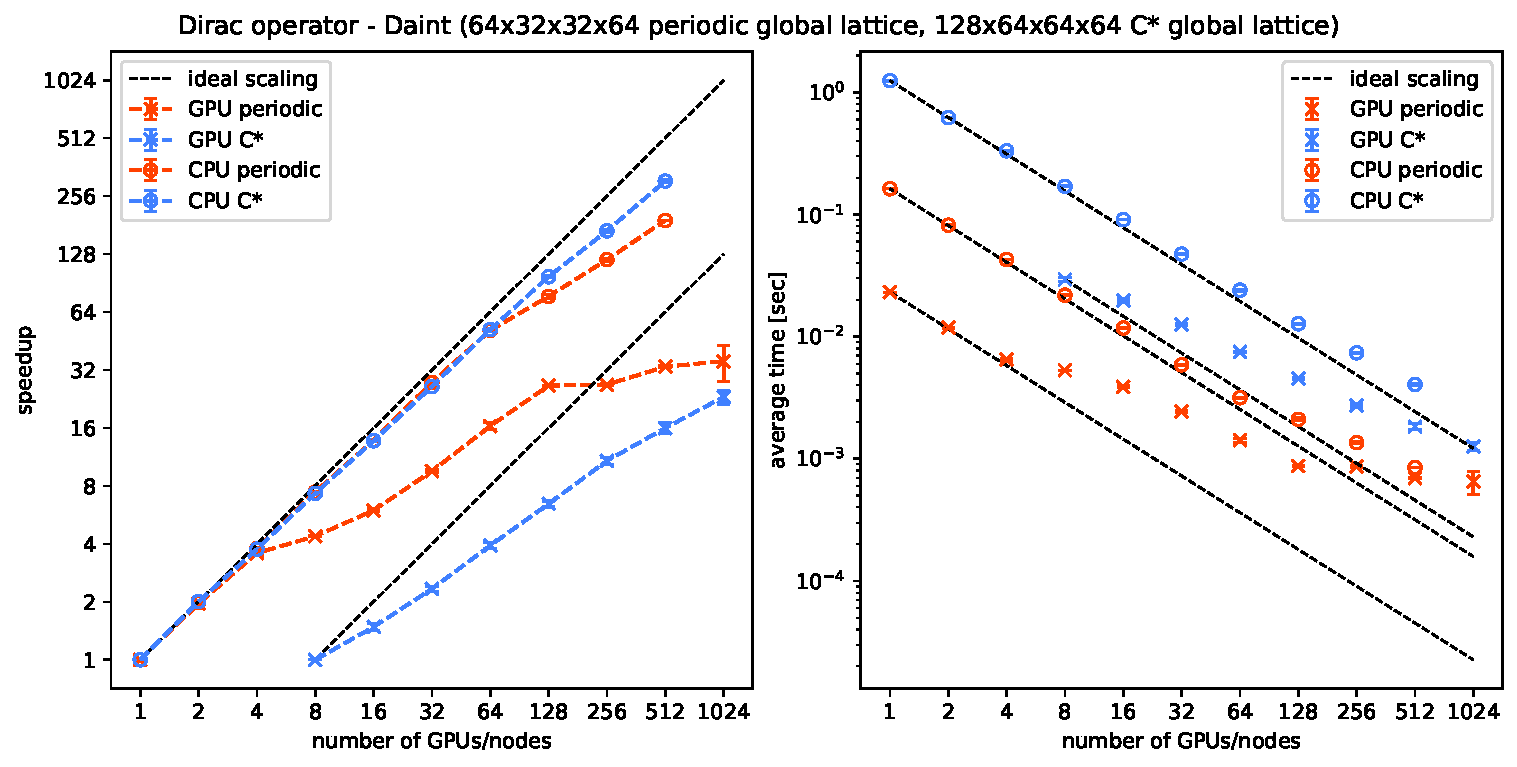
\includegraphics[width=\linewidth]{\dir/img/daint_dw_strong}
%     \caption{Strong scaling (left) and time for one application (right) of the Dirac operator on Piz Daint (see \cref{sec:hardware}) on the CPU (circles) and GPU (crosses) using a periodic (red) and a lattice with 3 C$^\star$ directions (blue). The x-axis denotes the number of nodes for CPU runs (32 ranks per node) and number of GPUs for GPU runs (1 P100 GPU per node). The global lattice sizes are $V_\mathrm{G} = (64 \times 32 \times 32 \times 64)$ and $V_\mathrm{G} = (64 \times 64 \times 64 \times 128)$ for the periodic and C$^\star$ runs, respectively.}
%     \label{fig:old:daint:dw:strong}
% \end{figure}

% \begin{figure}
%     \centering
%     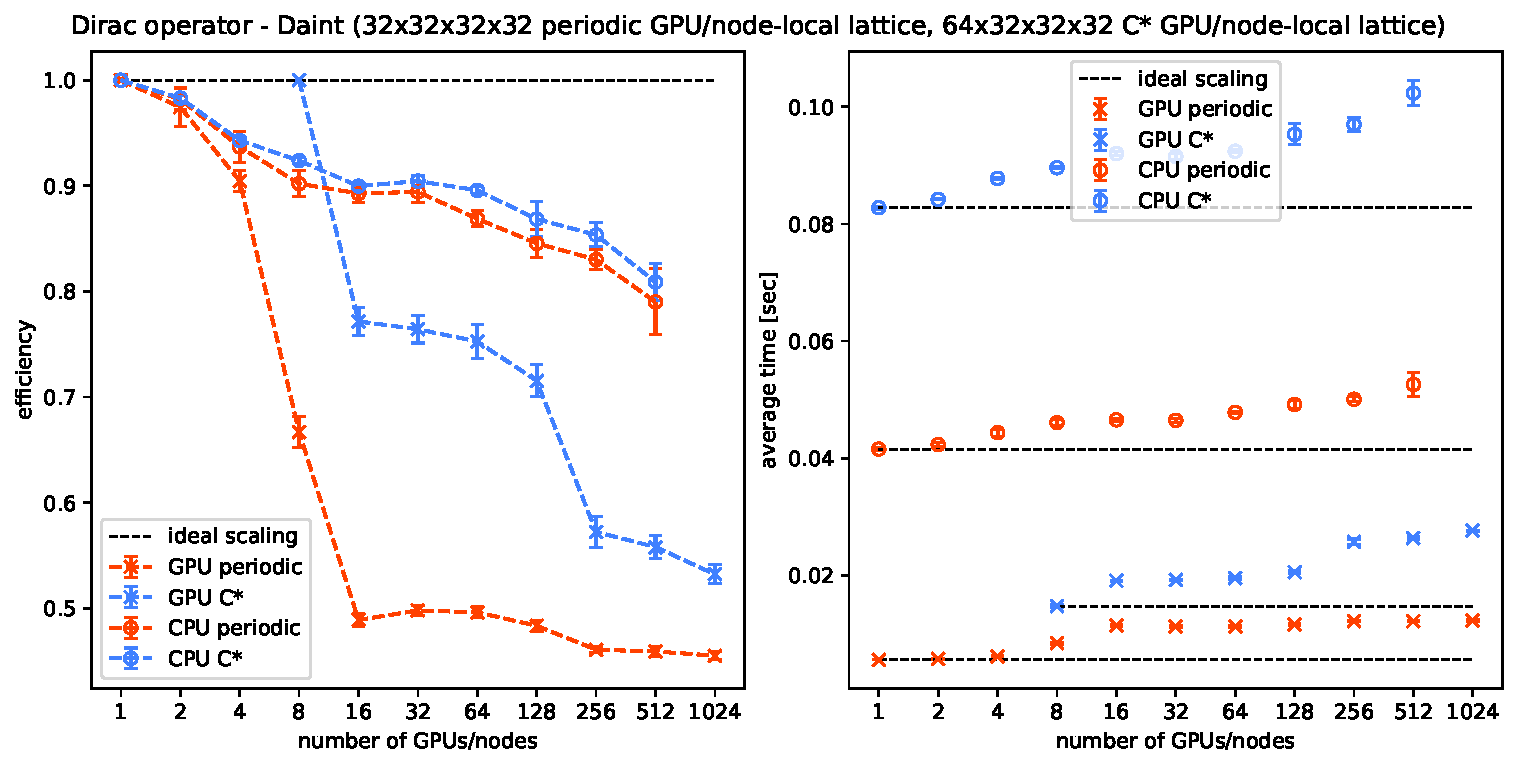
\includegraphics[width=\linewidth]{\dir/img/daint_dw_weak}
%     \caption{Weak scaling (left) and time for one application (right) of the Dirac operator on Piz Daint (see \cref{sec:hardware}), the setup is the same as in \cref{fig:old:daint:dw:strong}. The node- or GPU-local lattice sizes are $V_\mathrm{L} = (32 \times 32 \times 32 \times 32)$ and $V_\mathrm{L}= (64 \times 32 \times 32 \times 32)$ for the periodic and C$^\star$ runs, respectively. Notice that the physical lattice is of the same size in both cases (the C$^\star$ lattice needs to be doubled in one of the spatial directions).}
%     \label{fig:old:daint:dw:weak}
% \end{figure}

% \begin{figure}
%     \centering
%     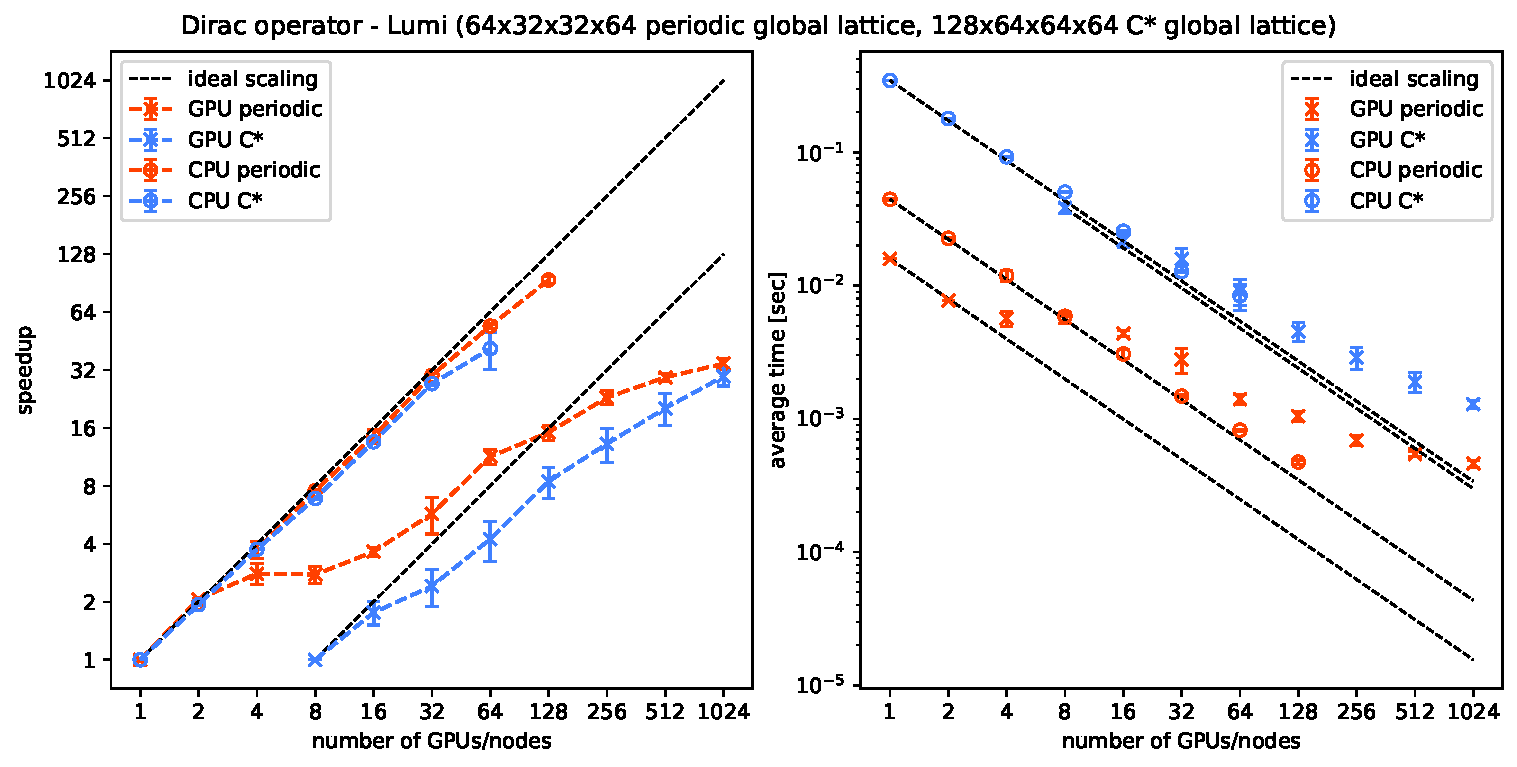
\includegraphics[width=\linewidth]{\dir/img/lumi_dw_strong}
%     \caption{Strong scaling (left) and time for one application (right) of the Dirac operator on LUMI-G and LUMI-C (see \cref{sec:hardware}). Notice that for the x-axis, number of GPUs is not the same as the number of nodes. A LUMI-G nodes has 4x AMD MI250s, logically abstracted as 8 GPUs.}
%     \label{fig:lumi:dw:strong}
% \end{figure}

% \begin{figure}
%     \centering
%     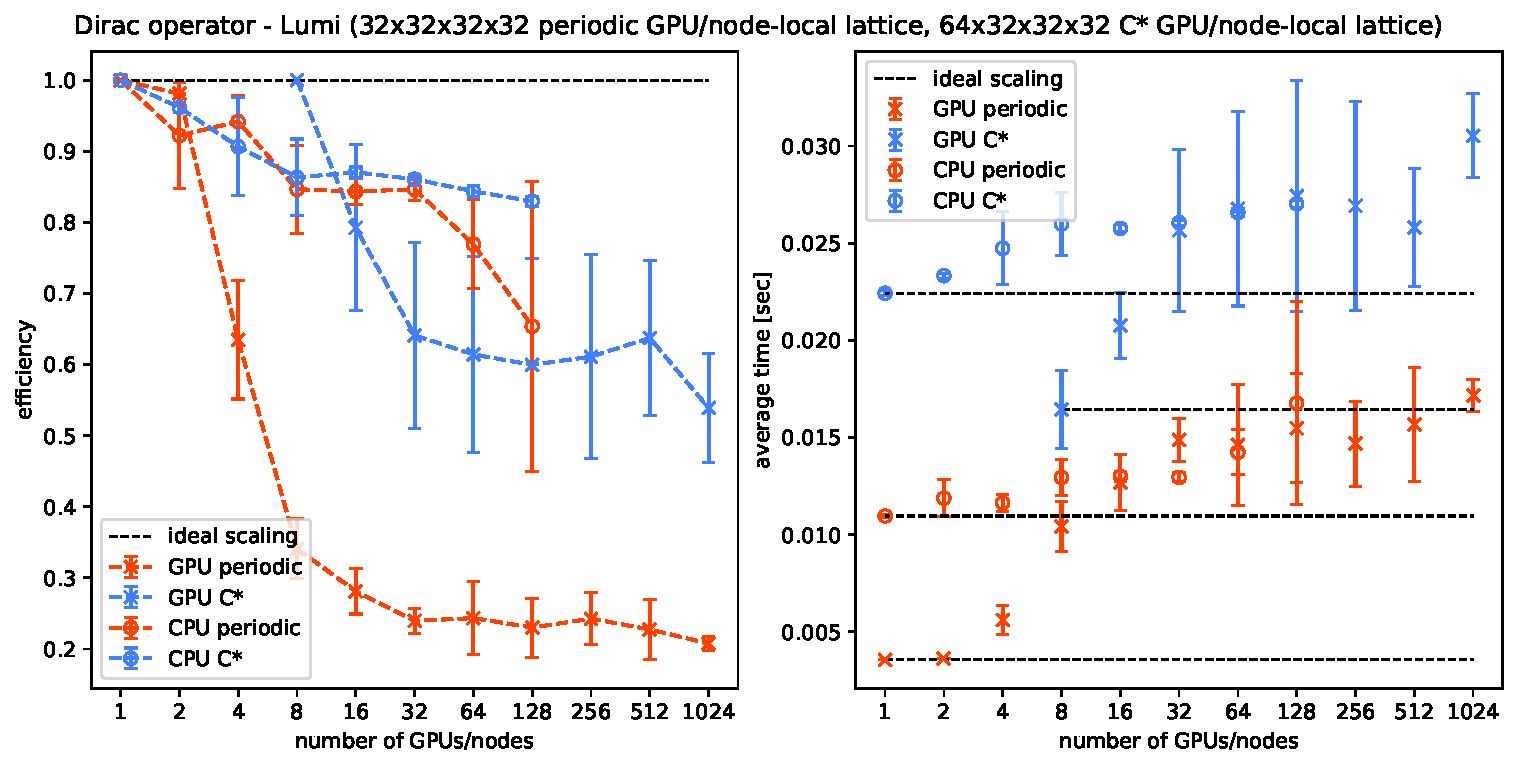
\includegraphics[width=\linewidth]{\dir/img/lumi_dw_weak}
%     \caption{Weak scaling (left) and time for one application (right) of the Dirac operator on LUMI-G (see \cref{sec:hardware}).}
%     \label{fig:lumi:dw:weak}
% \end{figure}

% \subsection{Solving the Dirac equation}

% For solving the Dirac equation, we use a heavily preconditioned GCR algorithm. In case of the CPU runs, we use openQxD's deflated mixed-precision%
% \footnote{single and double precision IEEE-754 floats} GCR solver that uses Schwarz alternating procedure as a preconditioner (\code{DFL\_SAP\_GCR} in openQCD parlance). The GPU runs use QUDAs mixed-precision%
% \footnote{half, single and double precision IEEE-754 floats} multi-grid GCR solver (MG). The two solvers are very similar in how they generate the coarse grid subspace. The CPU solver parameters are tuned, but due to lack of experience with multi-grid, we used a somewhat not optimised parameter set for multi-grid on the GPU. The relative residual is chosen to be $10^{-12}$ for all solves.

% We obtain good weak scaling, see \cref{fig:inv_weak}. Again, LUMI outperforms Piz Daint in terms of cost. This is expected, since one LUMI-G node contains $4$ AMD MI250s (abstracted as $8$ devices) and one Piz Daint hybrid node contains a single NVIDIA P100. The factor is not 4x, but rather $\ge10$x, which is explained by the higher memory bandwidth of the former GPU \footnote{P100: 720 GB/s \cite{online:nv_p100} vs. MI250: 3.2768 TB/s \cite{online:amd_mi250}.}.
% We note that strong-scaling for multi-grid algorithms is inherently challenging due to the reduced numbers of degrees of freedom on the coarser levels, which requires new algorithmic ideas~\cite{Espinoza-Valverde:2022pci}.

% % \begin{table}
% % \begin{tabular}{l|l|l}
% % \toprule
% %  & \multicolumn{2}{c}{cost in node-seconds [sec]} \\
% % \midrule
% % GPUs & LUMI-G & Piz Daint \\
% % \midrule
% %  32 & 34.6 &  347 \\
% %  64 & 70.0 &  748 \\
% % 128 & 159  & 1693 \\
% % 256 & 349  & 3584 \\
% % 512 & 825  & 8558 \\
% % \bottomrule
% % \end{tabular}
% % \caption{Cost in node-seconds of one solve of the Dirac equation. The GPU-local lattice is held constant ($V_\mathrm{L}=32x32x32x32$).}
% % \label{tab:nodehours_inv}
% % \end{table}

% \begin{figure}
%     \centering
%     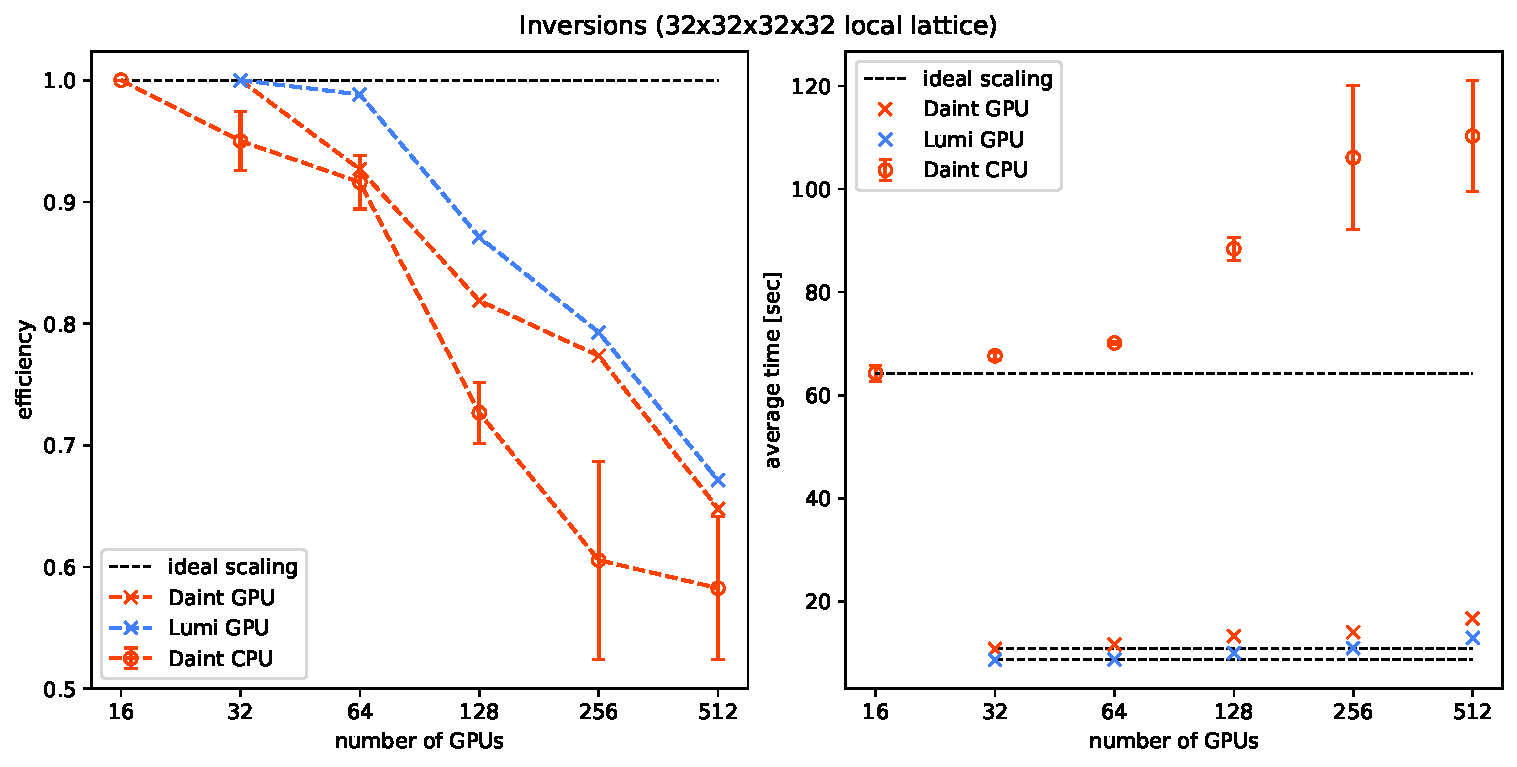
\includegraphics[width=\linewidth]{\dir/img/inv_weak}
%     \caption{Weak scaling (left) and time to solution (right) for one solve of the Dirac equation on LUMI (blue) and on Piz Daint (red) on the CPU (circle) and GPU (crosses) partition. For specifications on the machines, see \cref{sec:hardware}.}
%     \label{fig:inv_weak}
% \end{figure}

% }